\documentclass[11pt,a4paper]{article}
\usepackage{amsmath,amssymb}
\usepackage[margin=2.5cm]{geometry}
\usepackage{array}
\usepackage{bm}
\usepackage{graphicx}
\usepackage{booktabs}
\usepackage{xcolor}
\usepackage{tikz}
\usetikzlibrary{positioning,fit,backgrounds}
% Same convention as the paper's TikZ figures: blue = trained here, grey = frozen
% DA3-SMALL pretrained weights. Kept in sync with paper/main.tex's cTrain.
\definecolor{cTrain}{HTML}{4878CF}
\usepackage{hyperref}
\hypersetup{colorlinks=true, linkcolor=blue!50!black, urlcolor=blue!50!black}

% Long \texttt{} paths and \verb spans cannot hyphenate, so several of them spill
% into the right margin. Letting TeX stretch inter-word space as a last resort
% absorbs that instead of printing text past the text block.
\emergencystretch=6em

\title{Vision Mamba-3: Mamba-3 State-Space Duality as Attention,\\
       Its Non-Causal Extension to Images, and Four Applications}
\author{Masahiro Ogawa}
\date{\today}

\begin{document}
\maketitle

\begin{abstract}
This report derives, step by step, how the Mamba-3 state space model (SSM) can be
used as a drop-in replacement for both self-attention and cross-attention, extends
the result to images as \emph{Vision Mamba-3}, and measures the resulting operators
on four tasks. The derivation follows the notation of the original Mamba-3 paper so
every equation can be checked against the source, and every algebraic move is shown
with its justification. The structural claim throughout is that the SSD parallel
form $\bm{Y}=(\bm{L}\odot\bm{C}\bm{B}^\top)\bm{X}$ already has the shape of
attention, so putting it into a vision pipeline is a relabelling exercise plus a
mask-builder swap. On top of that we build the image operator: two positional
encodings (Mamba-3's own complex-SSM rotary, and an external 2-D RoPE applied to
$\bm{B}$ and $\bm{C}$), two- and four-directional scans, and the non-causal collapse
(VSSD-$\gamma$, called Visual State Space Duality --- VSSD --- in its source paper) that
removes causality without multi-scan. Four applications
follow --- segmentation-head design, CIFAR-10 classification, ETH3D camera pose, and
ETH3D metric depth --- each reported with the provenance of its numbers, including
the two studies whose honest answer is that the operator change alone did not help.
\end{abstract}

\tableofcontents

%% ================================================================
\section{Objective}
%% ================================================================
\label{sec:objective}

This report answers three questions about using Mamba-3 as an attention mechanism,
and keeps them separate because they have different kinds of answer.

\begin{enumerate}
  \item \textbf{Is the state-space duality literally attention?} This is a question
        of algebra, and the answer is exact. \S\ref{sec:notation} fixes notation and
        \S\ref{sec:ssd} derives
        $\bm{Y}=(\bm{L}\odot\bm{C}\bm{B}^\top)\bm{X}$ from the Mamba-3 recurrence,
        from which self-attention (\S\ref{sec:self}) and cross-attention
        (\S\ref{sec:cross}) follow by choosing which tokens supply
        $\bm{B},\bm{C},\bm{X}$.
  \item \textbf{What has to change to apply it to images?} An image has no causal
        order, so the causal mask that makes SSD efficient is exactly what makes it
        wrong here. \S\ref{sec:images} builds the image operator: where positional
        information enters (\S\ref{sec:rope}, \S\ref{sec:2drope}), how causality is
        removed either by scanning in several directions (\S\ref{sec:bidi},
        \S\ref{sec:4dir}) or by collapsing the mask outright (\S\ref{sec:ncssd}),
        what the tensor shapes actually are (\S\ref{sec:dimcheck}), and what the
        implementation commits to (\S\ref{sec:impl}).
  \item \textbf{Does it work on real tasks?} This is a question of measurement, and
        the answer is mixed. Four studies follow: segmentation-head design
        (\S\ref{sec:app-seg}), CIFAR-10 classification (\S\ref{sec:cifar}), ETH3D
        camera pose (\S\ref{sec:eth3d}), and ETH3D metric depth
        (\S\ref{sec:eth3d-depth}).
\end{enumerate}

\paragraph{On reading the measured numbers.} The derivations in
\S\ref{sec:notation}--\S\ref{sec:images} are checkable against \cite{mamba3} and do
not depend on any run. The numbers in \S\ref{sec:cifar}--\S\ref{sec:eth3d-depth} do,
and they were not all produced by the same version of the operator: 2-D RoPE, the
fused Triton kernel, and the pinned upstream submodule (\S\ref{sec:impl}) all landed
after some of the runs reported here. Where that is true it is stated at the table
rather than left for the reader to infer, because two of these tables disagree with
each other and the reason is provenance, not noise. Two results are negative and are
reported as such: on CIFAR-10 no state-space variant beats a small CNN at this data
scale, and on ETH3D pose both variants fail to beat un-patched zero-shot DA-3.

%% ================================================================
%% ================================================================
%% ================================================================
\section{Notation}
\label{sec:notation}
%% ================================================================

We summarize the symbols used throughout. The names match
\cite{mamba3}, Section~2 and Section~3.

\subsection{Sizes}\label{sec:sizes}

\begin{itemize}
  \item $T$: sequence length (number of tokens). For images we will
        set $T = L = HW/P^2$ where $H,W$ are the image height and
        width and $P$ is the patch size.
  \item $D$: model (channel) dimension.
  \item $N$: SSM state dimension (per SSM head).
  \item $R$: MIMO rank (Mamba-3, \S 3.3). For SISO, $R=1$.
  \item $d_{\text{head}}$: per-head channel width, $d_{\text{head}} =
        D/(\text{number of heads})$. The channels $D$ are split across
        several heads that each run their own SSM; the worked examples
        use $D=384$ over $6$ heads, so $d_{\text{head}}=64$.
  \item $m, k, n$: \emph{generic placeholder} dimensions used only when
        pricing the cost of a matrix product $(m\times k)\cdot(k\times
        n)$, where $k$ is the shared/contracted dimension that is summed
        over. They are not fixed model sizes: in each cost estimate we
        instantiate $m,k,n$ from $T$, $N$, and $d_{\text{head}}$.
\end{itemize}

\subsection{Tokens and projections}

\begin{itemize}
  \item $\bm{X} \in \mathbb{R}^{T\times D}$ is the input sequence;
        the $t$-th row $\bm{x}_t \in \mathbb{R}^{D}$ is one token.
  \item $\bm{B}, \bm{C} \in \mathbb{R}^{T\times N}$ are data-dependent
        projections; the $t$-th rows are $\bm{B}_t, \bm{C}_t \in
        \mathbb{R}^{N}$.
  \item $\Delta_t \in \mathbb{R}_{>0}$ is a data-dependent step size.
  \item $A_t \in \mathbb{R}_{<0}$ is a data-dependent (in Mamba-3) or
        data-independent (in Mamba-2) scalar that governs decay.
  \item $\bm{h}_t \in \mathbb{R}^{N}$ is the hidden state at time $t$
        (SISO; see \S\ref{sec:mimo} for MIMO).
  \item $\bm{Y} \in \mathbb{R}^{T\times D}$ is the output sequence.
\end{itemize}

In terms of an input token $\bm{x}_t$, the learned projections are
\begin{align}
  \bm{B}_t       &= \bm{W}_B\,\bm{x}_t  & \bm{W}_B &\in \mathbb{R}^{N\times D}, \label{eq:projB}\\
  \bm{C}_t       &= \bm{W}_C\,\bm{x}_t  & \bm{W}_C &\in \mathbb{R}^{N\times D}, \label{eq:projC}\\
  \Delta_t       &= \mathrm{Softplus}(\bm{w}_\Delta^\top \bm{x}_t)
                                         & \bm{w}_\Delta &\in \mathbb{R}^{D}, \label{eq:projD}\\
  A_t            &= -\mathrm{Softplus}(\bm{w}_A^\top \bm{x}_t)
                                         & \bm{w}_A &\in \mathbb{R}^{D} \text{ (optional data-dep.)}. \label{eq:projA}
\end{align}
Here $\mathrm{Softplus}$ is the smooth, strictly positive activation
\begin{equation}\label{eq:softplus}
  \mathrm{Softplus}(z) := \log\bigl(1 + e^{z}\bigr),
  \qquad \mathrm{Softplus}:\mathbb{R}\to\mathbb{R}_{>0},
\end{equation}
so \eqref{eq:projD} guarantees $\Delta_t > 0$ and \eqref{eq:projA}
guarantees $A_t < 0$, which is what the discretization in
\eqref{eq:abc} requires for $\alpha_t = e^{\Delta_t A_t} \in (0,1)$.

The value projection that we will feed into the SSM is
\begin{equation}\label{eq:projV}
  \bm{v}_t = \mathrm{SiLU}(\bm{W}_V\,\bm{x}_t),
  \qquad \bm{W}_V \in \mathbb{R}^{D\times D},
\end{equation}
where $\mathrm{SiLU}$ (a.k.a.\ Swish) is the smooth, self-gated activation
\begin{equation}\label{eq:silu}
  \mathrm{SiLU}(z) := z\,\sigma(z) = \frac{z}{1 + e^{-z}},
  \qquad
  \sigma(z) := \frac{1}{1 + e^{-z}},
\end{equation}
applied element-wise to the vector $\bm{W}_V\bm{x}_t \in \mathbb{R}^{D}$.

We also use $\mathrm{softmax}$ when comparing SSD to standard
attention. For a row vector $\bm{z}=(z_1,\dots,z_T)\in\mathbb{R}^{T}$,
\begin{equation}\label{eq:softmax}
  \mathrm{softmax}(\bm{z})_j \;:=\; \frac{e^{z_j}}{\sum_{k=1}^{T} e^{z_k}},
  \qquad j=1,\dots,T,
\end{equation}
so the entries of $\mathrm{softmax}(\bm{z})$ are non-negative and sum
to $1$. Applied to a matrix
$\bm{S}\in\mathbb{R}^{T\times T}$ as $\mathrm{softmax}(\bm{S})$, the
operator is taken \emph{row-wise} — each row of $\bm{S}$ is independently
mapped through \eqref{eq:softmax}, so each row of
$\mathrm{softmax}(\bm{S})$ sums to $1$. In standard scaled-dot-product
attention this is what enforces ``each query's attention weights form
a probability distribution over the keys'':
\[
  \bm{Y} \;=\; \mathrm{softmax}\!\bigl(\bm{Q}\bm{K}^\top/\sqrt{d}\bigr)\,\bm{V}.
\]
The Mamba-3 SSD parallel form \eqref{eq:ssd} replaces this row-wise
softmax with element-wise multiplication by a learned mask
$\bm{L}$, dropping both the exponential and the row normalisation.

\subsection{RMSNorm and BCNorm}
\label{sec:bcnorm}

Mamba-3 normalizes the key/query projections $\bm{B}_t,\bm{C}_t$ before
using them in the SSD kernel. The underlying primitive is
\emph{RMSNorm} \cite{rmsnorm}, which rescales a vector by its
root-mean-square (no mean subtraction, unlike LayerNorm):
\begin{equation}\label{eq:rmsnorm}
  \mathrm{RMSNorm}(\bm{u}) := \frac{\bm{u}}{\sqrt{\tfrac{1}{N}\sum_{i=1}^{N} u_i^{2} + \varepsilon}}\;\odot\;\bm{g},
  \qquad \bm{u}\in\mathbb{R}^{N},
\end{equation}
where $\bm{g}\in\mathbb{R}^{N}$ is a learnable per-channel gain,
$\varepsilon>0$ is a small constant, and $\odot$ is the Hadamard
product. The output has unit RMS up to the learned gain, which
stabilizes the inner products $\bm{C}_i^\top\bm{B}_j$ that appear in
\eqref{eq:ssd}.

\emph{BCNorm} (\cite{mamba3} \S 3.4) is simply RMSNorm applied
independently to $\bm{B}_t$ and $\bm{C}_t$, followed by a learnable
channel-wise bias:
\begin{equation}\label{eq:bcnorm}
  \bm{B}_t \leftarrow \mathrm{RMSNorm}(\bm{B}_t) + \bm{b}_B,
  \qquad
  \bm{C}_t \leftarrow \mathrm{RMSNorm}(\bm{C}_t) + \bm{b}_C,
  \qquad \bm{b}_B,\bm{b}_C \in \mathbb{R}^{N}.
\end{equation}
We will write ``apply BCNorm'' as shorthand for the substitution
\eqref{eq:bcnorm}; each occurrence of $\bm{B}_t,\bm{C}_t$ in later
equations is understood to be the post-BCNorm version when the
algorithm calls for it.

\subsection{Recurrence, parallel form, and decay factors}
\label{sec:decay}

Mamba-3 uses the \emph{exponential-trapezoidal} discrete recurrence of
\cite{mamba3} eq.~(5)–(6):
\begin{equation}\label{eq:rec3}
  \bm{h}_t = \alpha_t\,\bm{h}_{t-1}
            + \beta_t\,\bm{B}_{t-1}\bm{x}_{t-1}
            + \gamma_t\,\bm{B}_t\bm{x}_t,
  \qquad
  \bm{y}_t = \bm{C}_t^\top\bm{h}_t,
\end{equation}
with the three data-dependent scalars
\begin{equation}\label{eq:abc}
  \alpha_t := e^{\Delta_t A_t},
  \qquad
  \beta_t  := (1 - \lambda_t)\,\Delta_t\,e^{\Delta_t A_t},
  \qquad
  \gamma_t := \lambda_t\,\Delta_t,
\end{equation}
where $\lambda_t \in [0,1]$ is a learned, data-dependent convex weight.
Setting $\lambda_t \equiv 1$ recovers Mamba-2's two-term recurrence
\begin{equation}\label{eq:rec2}
  \bm{h}_t = \alpha_t\,\bm{h}_{t-1} + \gamma_t\,\bm{B}_t\,\bm{x}_t,
  \qquad
  \bm{y}_t = \bm{C}_t^\top\,\bm{h}_t,
\end{equation}
which is \cite{mamba3} eq.~(1). Mamba-3's \emph{parallel} form
(\cite{mamba3} eq.~(2)) reads
\begin{equation}\label{eq:ssd}
  \bm{Y} = \bigl(\bm{L}\odot\bm{C}\bm{B}^\top\bigr)\bm{X},
\end{equation}
with $\odot$ the Hadamard product and $\bm{L}\in\mathbb{R}^{T\times T}$
a structured lower-triangular mask that we derive explicitly in
Section~\ref{sec:ssd}. This single equation is the bridge between
recurrences and attention: the next section is devoted to explaining
exactly why. When the specific recurrence matters we write $\bm{L}_2$
for Mamba-2's two-term mask \eqref{eq:L2} and $\bm{L}_3$ for Mamba-3's
three-term (trapezoidal) mask \eqref{eq:L3}; unadorned $\bm{L}$ means
either, whichever is in scope.

\subsection{What this note actually does}

Using only the objects above, we will:

\begin{enumerate}
  \item Derive \eqref{eq:ssd} from \eqref{eq:rec2} and
        \eqref{eq:rec3}, and read it as \emph{linear attention with a
        learned mask} (Section~\ref{sec:ssd}).
  \item Plug real projections into \eqref{eq:ssd} to get a Mamba-3
        self-attention block (Section~\ref{sec:self}).
  \item Repeat for two different sequences and obtain Mamba-3 cross-
        attention, in two flavours: state-compressed (cheap,
        constant-memory) and token-level (exact SSD analogue of
        softmax cross-attention) (Section~\ref{sec:cross}).
  \item Patchify an image, make the scan bidirectional, and use the
        self/cross-attention blocks to build an image encoder; then
        combine several views via cross-view attention for the 3-D
        setting (Section~\ref{sec:images}).
  \item Derive the non-causal collapse \emph{VSSD-$\gamma$} of \cite{vssd}
        as an algebraic alternative to bidirectional scans, and show
        that it collapses the structured $T\times T$ mask $\bm{L}$ to
        a single learned $T$-vector $\bm{m}$
        (Section~\ref{sec:ncssd}).
\end{enumerate}

%% ================================================================
%% ================================================================
%% ================================================================
\section{State-Space Duality}
\label{sec:ssd}
%% ================================================================

We derive \eqref{eq:ssd} directly from the recurrence. Work entirely
with the two-term form \eqref{eq:rec2} first; the three-term form
\eqref{eq:rec3} is a corollary (\S\ref{sec:trap}).

%% ================================================================
\subsection{SSD is already attention (the result up front)}
%% ================================================================

The Structured State-space Duality (Dao~\&~Gu 2024; Lahoti et al.\
2026) shows that the Mamba SSD parallel form and softmax attention
share an output shape:
\begin{equation}\label{eq:duality}
  \underbrace{\bm{Y} = \bigl(\bm{L}\odot\bm{C}\bm{B}^\top\bigr)\bm{V}}_{\text{Mamba SSD (2 or 3)}}
  \qquad\Longleftrightarrow\qquad
  \underbrace{\bm{Y} = \mathrm{softmax}\!\bigl(\bm{Q}\bm{K}^\top/\sqrt{d}\bigr)\bm{V}}_{\text{softmax attention}}.
\end{equation}
Matching by shape gives the substitution
\[
  \bm{Q} \leftarrow \bm{C},\qquad
  \bm{K} \leftarrow \bm{B},\qquad
  \bm{V} \leftarrow \mathrm{SiLU}(\bm{W}_V\bm{x}),
\]
i.e.\ query and key projections are the SSD $\bm{C}$ and $\bm{B}$
streams; the value projection is the same learned $\bm{W}_V$ that
softmax attention uses (this is shared with Mamba-2; Mamba-3 only
changes the structure of $\bm{L}$). The only structural difference
from softmax attention is that the row-wise normalisation
$\mathrm{softmax}(\cdot/\sqrt{d})$ is replaced by an element-wise
multiplication by the learned, structured mask $\bm{L}$.

For Mamba-3 the trapezoidal three-term recurrence introduces a richer
$\bm{L}$ (two contributions per $(t,j)$ cell), but does not change the
shape of \eqref{eq:duality}. For the \emph{non-causal} variant
(VSSD, Shi et al.\ 2025), the $T\times T$ mask collapses to a
$T$-vector $\bm{m}$ and the formula simplifies further to
\begin{equation}\label{eq:vssd}
  \bm{Y} \;=\; \bm{C}\,\bigl((\bm{B}\odot\bm{m})^\top\bm{X}\bigr),
\end{equation}
a single global $N\times d$ hidden state, no mask materialization.
The derivation is \S\ref{sec:ssd-unroll}--\S\ref{sec:trap} below.

\subsection{Unrolling the two-term recurrence}
\label{sec:ssd-unroll}

Starting from $\bm{h}_0 = \bm{0}$ and applying \eqref{eq:rec2} once:
\begin{equation}\label{eq:un1}
  \bm{h}_1 = \alpha_1\,\bm{h}_0 + \gamma_1\,\bm{B}_1\bm{x}_1
           = \gamma_1\,\bm{B}_1\bm{x}_1.
\end{equation}
Apply it once more:
\begin{align}
  \bm{h}_2 &= \alpha_2\,\bm{h}_1 + \gamma_2\,\bm{B}_2\bm{x}_2 \nonumber \\
           &= \alpha_2\,\gamma_1\,\bm{B}_1\bm{x}_1
             + \gamma_2\,\bm{B}_2\bm{x}_2. \label{eq:un2}
\end{align}
By induction on $t$ we claim
\begin{equation}\label{eq:un-claim}
  \bm{h}_t \;=\; \sum_{j=1}^{t}
     \underbrace{\Bigl(\prod_{k=j+1}^{t}\alpha_k\Bigr)}_{=:\,a_{t\leftarrow j}}
     \gamma_j\,\bm{B}_j\bm{x}_j,
\end{equation}
where by convention an empty product equals $1$ (so
$a_{t\leftarrow t} = 1$).

\emph{Proof of the induction step.} Assume \eqref{eq:un-claim} at
time $t-1$. Substitute into \eqref{eq:rec2}:
\begin{align}
  \bm{h}_t
   &= \alpha_t\,\bm{h}_{t-1} + \gamma_t\,\bm{B}_t\bm{x}_t \\
   &= \alpha_t \sum_{j=1}^{t-1}
        \Bigl(\prod_{k=j+1}^{t-1}\alpha_k\Bigr)\gamma_j\bm{B}_j\bm{x}_j
        + \gamma_t\,\bm{B}_t\bm{x}_t \\
   &= \sum_{j=1}^{t-1}
        \Bigl(\prod_{k=j+1}^{t}\alpha_k\Bigr)\gamma_j\bm{B}_j\bm{x}_j
        + \gamma_t\,\bm{B}_t\bm{x}_t
        \qquad\text{(absorb $\alpha_t$ into the product)}\\
   &= \sum_{j=1}^{t}
        \Bigl(\prod_{k=j+1}^{t}\alpha_k\Bigr)\gamma_j\bm{B}_j\bm{x}_j.
\end{align}
The last equality uses the empty-product convention for $j=t$. This
proves \eqref{eq:un-claim}.

\subsection{From state to output}

Plug \eqref{eq:un-claim} into the output equation
$\bm{y}_t = \bm{C}_t^\top\bm{h}_t$:
\begin{align}
  \bm{y}_t
   &= \bm{C}_t^\top \sum_{j=1}^{t}
        a_{t\leftarrow j}\,\gamma_j\,\bm{B}_j\bm{x}_j \\
   &= \sum_{j=1}^{t}
        a_{t\leftarrow j}\,\gamma_j\,
        \underbrace{\bm{C}_t^\top \bm{B}_j}_{\text{scalar}}\;\bm{x}_j
        \qquad\text{(linearity of $\bm{C}_t^\top(\cdot)$)} \label{eq:yout} \\
   &= \sum_{j=1}^{t}
        \underbrace{\bigl(a_{t\leftarrow j}\,\gamma_j\bigr)}_{=:\,L_{tj}}
        \bigl(\bm{C}_t^\top \bm{B}_j\bigr)\,\bm{x}_j. \label{eq:yout-L}
\end{align}
The key observation is that $\bm{x}_j$ is a vector while
$\bm{C}_t^\top\bm{B}_j$ is a scalar; we are free to reorder the
factors.

\subsection{Matrix form: \texorpdfstring{$\bm{Y} = (\bm{L}\odot \bm{C}\bm{B}^\top)\bm{X}$}{Y = (L .* C B-transpose) X}}

Define the lower-triangular matrix
\begin{equation}\label{eq:L2}
  L_{tj} \;=\;
  \begin{cases}
     \gamma_j\displaystyle\prod_{k=j+1}^{t}\alpha_k & j \le t,\\[4pt]
     0 & j > t.
  \end{cases}
\end{equation}
Equivalently,
\begin{equation}\label{eq:Lmat}
  \bm{L} \;=\;
  \begin{bmatrix}
     1    &      &       &      \\
     \alpha_2 & 1 &       &      \\
     \alpha_3\alpha_2 & \alpha_3 & 1 &   \\
     \vdots & & \ddots & \\
     \prod_{k=2}^{T}\alpha_k & \cdots & \alpha_T & 1
  \end{bmatrix}\cdot\mathrm{diag}(\gamma_1,\dots,\gamma_T),
\end{equation}
which is the Mamba-2 mask of \cite{mamba3} eq.~(3). Using
\eqref{eq:yout-L} row by row,
\begin{equation}\label{eq:rowform}
  \bm{y}_t \;=\; \sum_{j=1}^{T} L_{tj}\,\bigl(\bm{C}_t^\top \bm{B}_j\bigr)\,\bm{x}_j
         \;=\; \sum_{j=1}^{T}
                \bigl[\,\bm{L}\odot\bm{C}\bm{B}^\top\,\bigr]_{tj}\,\bm{x}_j.
\end{equation}
(Terms with $j>t$ vanish because $L_{tj}=0$.) Stacking over $t$,
\begin{equation}\label{eq:ssd-derived}
  \boxed{\;\bm{Y} \;=\; \bigl(\bm{L}\odot \bm{C}\bm{B}^\top\bigr)\bm{X}.\;}
\end{equation}
This is exactly \eqref{eq:ssd} (\cite{mamba3} eq.~(2)).

\subsection{Reading the SSD identity as linear attention}

Define the standard attention quantities
\begin{equation}
  \bm{Q}_t := \bm{C}_t,\qquad \bm{K}_j := \bm{B}_j,\qquad \bm{V}_j := \bm{x}_j.
\end{equation}
Then \eqref{eq:ssd-derived} is
\begin{equation}\label{eq:attn}
  \bm{Y} \;=\; \bigl(\bm{L}\odot \bm{Q}\bm{K}^\top\bigr)\bm{V},
\end{equation}
which is \emph{linear attention} (no softmax, no row normalization),
with a data-dependent, structured mask $\bm{L}$. Compare to standard
softmax self-attention
$\bm{Y} = \mathrm{softmax}(\bm{Q}\bm{K}^\top / \sqrt{d})\,\bm{V}$:
\begin{itemize}
  \item Standard attention computes a dense $T\times T$ similarity
        matrix $\bm{Q}\bm{K}^\top$ and row-normalizes it by softmax.
  \item Mamba-3 SSD computes the same $\bm{Q}\bm{K}^\top$, then
        multiplies it elementwise by a learned mask $\bm{L}$ whose
        off-diagonal entries decay geometrically in $|t-j|$.
  \item The decay factor $\prod_{k=j+1}^{t}\alpha_k$ plays the role of
        a relative-position bias: tokens separated by large
        $\sum_{k}\Delta_k |A_k|$ contribute exponentially less.
\end{itemize}

\subsection{Trapezoidal three-term form}\label{sec:trap}

The same derivation goes through for \eqref{eq:rec3}. We show only
the new piece: the mask acquires an extra two-band contribution.
Substitute \eqref{eq:rec3} once,
\begin{align}
  \bm{h}_t
   &= \alpha_t\,\bm{h}_{t-1}
     + \beta_t\,\bm{B}_{t-1}\bm{x}_{t-1}
     + \gamma_t\,\bm{B}_t\bm{x}_t.
\end{align}
Iterating (compare \eqref{eq:un-claim}) gives
\begin{equation}\label{eq:un3}
  \bm{h}_t = \sum_{j=1}^{t}
     \Bigl(\prod_{k=j+1}^{t}\alpha_k\Bigr)\!\bigl(\gamma_j\,\bm{B}_j\bm{x}_j
                                               + \beta_j\,\bm{B}_{j-1}\bm{x}_{j-1}\bigr),
\end{equation}
where the $\beta_j$ term contributes to the state via
$\bm{B}_{j-1}\bm{x}_{j-1}$. Plugging into
$\bm{y}_t = \bm{C}_t^\top\bm{h}_t$ and collecting coefficients of
$\bm{B}_j\bm{x}_j$ (note the index shift for the $\beta$ term), one
obtains
\begin{equation}\label{eq:L3}
  L_{tj} \;=\; \Bigl(\prod_{k=j+1}^{t}\alpha_k\Bigr)\gamma_j
            \;+\; \Bigl(\prod_{k=j+2}^{t}\alpha_k\Bigr)\beta_{j+1}
            \quad \text{for } j\le t,
\end{equation}
with the usual empty-product convention. In matrix form this is
\cite{mamba3} eq.~(7): $\bm{L}$ is the product of a
1-semiseparable matrix (whose $(t,j)$ entry is
$\prod_{k=j+1}^{t}\alpha_k$) and a two-band matrix
$\mathrm{diag}(\gamma_0,\dots,\gamma_T) + \mathrm{subdiag}(\beta_1,\dots,\beta_T)$.
Equations \eqref{eq:rowform}–\eqref{eq:ssd-derived} are unchanged.

\paragraph{Boundary conditions of the $\beta$ band.} The second term in
\eqref{eq:L3} references $\beta_{j+1}$. For the left endpoint, the
recurrence \eqref{eq:rec3} at $t=1$ uses $\beta_1 \bm{B}_0\bm{x}_0$
with $\bm{B}_0, \bm{x}_0$ out of range; we therefore adopt the
convention $\beta_1 := 0$, or equivalently drop this term when
$t=1$. Consistently, $\beta_1$ never appears in \eqref{eq:L3}: the
second term at $j=0$ would need $\beta_1$, but $j\ge 1$ by indexing.
For the right endpoint, at $j=t$ the expression $\beta_{j+1}=\beta_{t+1}$
is undefined; we set $\beta_{T+1} := 0$ so the second term vanishes
at $j=t$, leaving $L_{tt} = \gamma_t$ as expected. Any implementation
that pads $\beta$ with zeros on both ends and builds the second band
only for the strictly lower triangle ($j<t$) honours both conventions
automatically. An off-by-one in this shift is silently masked by the
test $\lambda_t\equiv 1$ (which zeroes $\beta$ identically) and must
therefore be caught by an independent test with $\lambda_t \in (0,1)$.

%% ================================================================
%% ================================================================
%% ================================================================
\section{Mamba-3 Self-Attention}
\label{sec:self}
%% ================================================================

We now instantiate the duality \eqref{eq:ssd-derived} as a concrete
self-attention block for a single sequence
$\bm{X}\in\mathbb{R}^{T\times D}$.

\paragraph{Bridge from eq.~\eqref{eq:ssd-derived} to the attention form $\bm{Y} = (\bm{L}\odot\bm{C}\bm{B}^\top)\bm{V}$.}
The SSD identity $\bm{Y} = (\bm{L}\odot\bm{C}\bm{B}^\top)\bm{X}$ was
derived in \S\ref{sec:ssd} for the recurrence
\eqref{eq:rec3}, in which the symbol $\bm{x}_t$ stands for
\emph{whatever sequence is fed into the recurrence}. The symbol
$\bm{X}$ in \eqref{eq:ssd-derived} is therefore a \emph{placeholder
for the kernel's input matrix}, not a name reserved for the raw
patch-embedding sequence. In a Mamba-3 \emph{attention} block the
architectural choice is to feed not the raw token but the
value-projected vector $\bm{v}_t = \mathrm{SiLU}(\bm{W}_V\bm{x}_t)$
\eqref{eq:projV} into the recurrence:
\begin{equation}\label{eq:ssd-bridge-rec}
  \bm{h}_t \;=\; \alpha_t\bm{h}_{t-1} + \beta_t\bm{B}_{t-1}\bm{v}_{t-1}
                                       + \gamma_t\bm{B}_t\bm{v}_t,
  \qquad
  \bm{y}_t \;=\; \bm{C}_t^\top\bm{h}_t.
\end{equation}
The unrolling of \S\ref{sec:ssd} did not depend on what the input is
called — only that the recurrence has the shape \eqref{eq:rec3} — so
\eqref{eq:ssd-bridge-rec} unrolls to exactly \eqref{eq:ssd-derived}
with $\bm{X}$ replaced by $\bm{V}$:
\begin{equation}\label{eq:self-bridge}
  \boxed{\;\bm{Y}_{\text{self}} \;=\; \bigl(\bm{L}\odot\bm{C}\bm{B}^\top\bigr)\bm{V},\;}
  \qquad
  \bm{V} := (\bm{v}_1,\dots,\bm{v}_T)^\top\in\mathbb{R}^{T\times D}.
\end{equation}
This is the same identity \eqref{eq:ssd-derived}, applied to the
specific input the block hands the kernel.

Placing self-attention next to softmax attention:
\[
  \underbrace{\bm{Y} = \bigl(\bm{L}\odot\bm{C}\bm{B}^\top\bigr)\bm{V}}_{\text{Mamba SSD (2 or 3)}}
  \qquad\Longleftrightarrow\qquad
  \underbrace{\bm{Y} = \mathrm{softmax}\!\bigl(\bm{Q}\bm{K}^\top/\sqrt{d}\bigr)\bm{V}}_{\text{softmax attention}},
\]
the substitution
\[
  \bm{Q} \;\leftarrow\; \bm{C},\qquad
  \bm{K} \;\leftarrow\; \bm{B},\qquad
  \bm{V} \;\leftarrow\; \mathrm{SiLU}(\bm{W}_V\bm{x}),
\]
makes the analogy literal: the \emph{query} projection becomes
$\bm{C}$ and the \emph{key} projection becomes $\bm{B}$; the value
$\bm{V}$ is the same one softmax attention uses. The only
structural difference is that row normalisation
$\mathrm{softmax}(\cdot/\sqrt{d})$ has been replaced by an
element-wise multiplication by the learned, structured mask $\bm{L}$.
That is the whole operator: pick the right $\bm{Q}/\bm{K}/\bm{V}$,
build $\bm{L}$ from the per-token scalars, multiply.

\paragraph{The trapezoidal three-term form does not change this shape.}
A reasonable worry: Mamba-3's three-term recurrence \eqref{eq:rec3}
adds a $\beta_t$ band that mixes adjacent tokens, so does the output
formula still factor as $\bm{Y} = (\bm{L}\odot\bm{C}\bm{B}^\top)\bm{V}$?
It does — only the \emph{contents} of $\bm{L}$ change.
\S\ref{sec:trap} derived this already: collecting coefficients of
$\bm{B}_j\bm{x}_j$ in the unrolled three-term state gives
\eqref{eq:L3},
\[
  L_{tj} = \Bigl(\prod_{k=j+1}^{t}\alpha_k\Bigr)\gamma_j
  \;+\; \Bigl(\prod_{k=j+2}^{t}\alpha_k\Bigr)\beta_{j+1},
\]
i.e.\ \emph{two} contributions per $(t,j)$ cell instead of one. The
Mamba-2 two-term mask \eqref{eq:L2} is exactly the special case
$\beta\equiv 0$ (equivalently $\lambda_t\equiv 1$). Plugging this
richer $L_{tj}$ into the same row formula \eqref{eq:rowform}
reproduces $\bm{Y} = (\bm{L}\odot\bm{C}\bm{B}^\top)\bm{V}$ unchanged;
only the mask gets an extra band. Consequence for an implementer:
Mamba-3 self-attention reuses every line of code that handles
Mamba-2 SSD, with the single change of swapping the mask builder
from a two-term to a three-term constructor.

\subsection{Per-token projections}

For each $t\in\{1,\dots,T\}$ compute
\begin{align}
  \bm{B}_t &= \bm{W}_B\,\bm{x}_t        & &\text{(key)} \\
  \bm{C}_t &= \bm{W}_C\,\bm{x}_t        & &\text{(query)} \\
  \Delta_t &= \mathrm{Softplus}(\bm{w}_\Delta^\top\bm{x}_t) & &\text{(step size)}\\
  A_t &= -\mathrm{Softplus}(\bm{w}_A^\top\bm{x}_t) \text{ or const.} & &\text{(decay)} \\
  \lambda_t &= \sigma(\bm{w}_\lambda^\top\bm{x}_t)\in[0,1] & &\text{(trapezoidal weight)} \\
  \bm{v}_t &= \mathrm{SiLU}(\bm{W}_V\,\bm{x}_t)         & &\text{(value)}
\end{align}
Form $\alpha_t,\beta_t,\gamma_t$ from \eqref{eq:abc}. Optionally apply
\textbf{BCNorm} (RMSNorm on $\bm{B}_t,\bm{C}_t$; \cite{mamba3}
\S 3.4) and learnable channel-wise biases $\bm{b}_B, \bm{b}_C$ before
using them.

\subsection{Self-attention output}

Assemble $\bm{B},\bm{C}\in\mathbb{R}^{T\times N}$ and the
value-projected matrix
$\bm{V} = (\bm{v}_1,\dots,\bm{v}_T)^\top\in\mathbb{R}^{T\times D}$
with rows $\bm{v}_t = \mathrm{SiLU}(\bm{W}_V\bm{x}_t)$
\eqref{eq:projV}, and the mask
$\bm{L}$ from \eqref{eq:L2} or \eqref{eq:L3}. The self-attention
output is
\begin{equation}\label{eq:self-out}
  \bm{Y}_{\text{self}} \;=\; \bigl(\bm{L}\odot\bm{C}\bm{B}^\top\bigr)\bm{V},
\end{equation}
or, entrywise,
\begin{equation}\label{eq:self-entry}
  \bm{y}_i^{\text{self}} \;=\; \sum_{j=1}^{i} L_{ij}\,(\bm{C}_i^\top \bm{B}_j)\,\bm{v}_j.
\end{equation}
Because $L_{ij}=0$ for $j>i$, the attention is \emph{causal}: token
$i$ sees tokens $1,\dots,i$. We remove this causality in
Section~\ref{sec:images} by running a second pass in the reverse
direction.

\subsection{MIMO extension}\label{sec:mimo}

Mamba-3's MIMO variant (\cite{mamba3} \S 3.3, eqs.~(12)–(14))
stacks $R$ parallel SSMs that share the scalar gates $\alpha_t,\Delta_t$
but carry independent $\bm{B}_t^{(j)},\bm{C}_t^{(i)},\bm{x}_t^{(j)}$.
The head-level output is
\begin{equation}
  \bm{y}_t^{(i)} \;=\; \sum_{j=0}^{R-1}\mathrm{SSM}\bigl(\alpha,\Delta,\bm{B}^{(j)},\bm{C}^{(i)},\bm{x}^{(j)}\bigr)_t,
\end{equation}
i.e.\ $R^2$ SISO calls in parallel. Using \eqref{eq:ssd-derived} on
each, the MIMO self-attention output is
\begin{equation}\label{eq:mimo-self}
  \bm{Y}^{(i)} \;=\; \sum_{j=0}^{R-1}
     \bigl(\bm{L}\odot \bm{C}^{(i)}\bm{B}^{(j)\top}\bigr)\bm{X}^{(j)},
  \quad i=0,\dots,R-1.
\end{equation}
This is exactly multi-head linear attention with shared mask.

%% ================================================================
%% ================================================================
%% ================================================================
\section{Mamba-3 Cross-Attention}
\label{sec:cross}
%% ================================================================

For cross-attention we have two token sequences: a \emph{query}
sequence $\bm{X}^{q}\in\mathbb{R}^{T_q\times D}$ and a \emph{key/value}
(context) sequence $\bm{X}^{kv}\in\mathbb{R}^{T_{kv}\times D}$.

\paragraph{Why cross-attention needs no new derivation.}
Cross-attention reuses the same identity, just with two different
sequences feeding the two sides instead of one. Place the two
formulas side by side:
\[
  \underbrace{\bm{Y} = \bigl(\bm{L}^{\text{cross}}\odot\bm{C}^q\bm{B}^{kv\top}\bigr)\bm{V}^{kv}}_{\text{Mamba-3 cross-SSD}}
  \qquad\Longleftrightarrow\qquad
  \underbrace{\bm{Y} = \mathrm{softmax}\!\bigl(\bm{Q}\bm{K}^\top/\sqrt{d}\bigr)\bm{V}}_{\text{softmax cross-attention}},
\]
with the substitution
\[
  \bm{Q} \;\leftarrow\; \bm{C}^q, \quad
  \bm{K} \;\leftarrow\; \bm{B}^{kv}, \quad
  \bm{V} \;\leftarrow\; \bm{V}^{kv} \;=\; \mathrm{SiLU}(\bm{W}_V \bm{x}^{kv}).
\]
The cross-attention output equation arises from
\eqref{eq:ssd-derived} by the same bridge as
\eqref{eq:self-bridge}: the input to the SSD kernel is the kv-side
value matrix
$\bm{V}^{kv}\in\mathbb{R}^{T_{kv}\times D}$, so the placeholder
$\bm{X}$ in \eqref{eq:ssd-derived} is filled by $\bm{V}^{kv}$.
The reading rule: the \emph{query} projection comes from the
query-side tokens $\bm{x}^{q}$, while \emph{both} the key and the
value projections come from the kv-side tokens $\bm{x}^{kv}$.
Nothing about the operator changes — only which sequence each
projection reads from.

\paragraph{Two things that do change relative to self-attention.}
First, the mask $\bm{L}^{\text{cross}}$ \eqref{eq:Lcross} is
rectangular ($T_q \times T_{kv}$) rather than triangular, because
queries and keys live on different time axes and there is no notion
of one token coming "before" another across the two streams.
Second, the trapezoidal structure of \eqref{eq:L3} carries over to
the kv axis when the kv side is itself produced by a Mamba-3
recurrence (the typical case in Variant~B, \S\ref{sec:crossB}): each
column of $\bm{L}^{\text{cross}}$ then has the same two-band decay
profile as a self-SSD row, with the recency bias discussed in
\S\ref{sec:crossB}. The output formula $\bm{Y} =
(\bm{L}^{\text{cross}}\odot\bm{C}^q\bm{B}^{kv\top})\bm{V}^{kv}$ is
\emph{unchanged}; only the geometry of $\bm{L}$ and which tokens
supply $\bm{C}, \bm{B}, \bm{V}$ are different. Consequence for an
implementer: cross-attention reuses every line of code that handles
self-SSD, with two changes — feed $\bm{C}$ from the query sequence
and $\bm{B}, \bm{V}$ from the kv sequence, and swap the
triangular mask builder for the rectangular \texttt{cross} mask.

\subsection{Projections for the two sides}

Query side:
\begin{equation}\label{eq:cross-proj-q}
  \bm{C}_i^{q} = \bm{W}_C\,\bm{x}_i^{q},
  \quad i=1,\dots,T_q,
\end{equation}
that is, only the \emph{query} projection is taken from the query
side. Key/value side:
\begin{align}
  \bm{B}_j^{kv} &= \bm{W}_B\,\bm{x}_j^{kv}, \\
  \Delta_j^{kv} &= \mathrm{Softplus}(\bm{w}_\Delta^\top \bm{x}_j^{kv}), \\
  A_j^{kv}      &= -\mathrm{Softplus}(\bm{w}_A^\top \bm{x}_j^{kv})\;\text{or const.}, \\
  \bm{v}_j^{kv} &= \mathrm{SiLU}(\bm{W}_V\,\bm{x}_j^{kv}),
  \quad j=1,\dots,T_{kv}.
\end{align}
Decay scalars $\alpha_j^{kv}$ etc.\ are computed as in \eqref{eq:abc}
but using the $kv$-side $\Delta_j^{kv}, A_j^{kv}$.

\subsection{Variant A: state-compressed cross-attention (constant memory)}
\label{sec:crossA}

Run the Mamba-3 recurrence \eqref{eq:rec2} on the $kv$-side with
\emph{outer-product} accumulation, treating $\bm{v}_j^{kv}$ as the
input instead of $\bm{x}_j^{kv}$. Define a matrix-valued hidden state
$\bm{H}_j \in \mathbb{R}^{N\times D}$ by
\begin{equation}\label{eq:Hrec}
  \bm{H}_j \;=\; \alpha_j^{kv}\,\bm{H}_{j-1}
                + \gamma_j^{kv}\,\bm{B}_j^{kv}\,\bm{v}_j^{kv\,\top},
  \qquad \bm{H}_0 = \bm{0}.
\end{equation}
By the exact same unrolling as in \eqref{eq:un-claim} we obtain
\begin{equation}\label{eq:Hclose}
  \bm{H}_{T_{kv}} \;=\; \sum_{j=1}^{T_{kv}}
      \Bigl(\prod_{k=j+1}^{T_{kv}}\alpha_k^{kv}\Bigr)
      \gamma_j^{kv}\,\bm{B}_j^{kv}\,\bm{v}_j^{kv\,\top}
  \;=:\; \bm{h}_{\text{ref}} \in \mathbb{R}^{N\times D}.
\end{equation}
This $\bm{h}_{\text{ref}}$ is the \emph{compressed context}: it
condenses the entire $kv$-sequence into a single $N\times D$ matrix.
For each query $\bm{C}_i^q$, the output is obtained by a single
left-multiplication:
\begin{equation}\label{eq:crossA-out}
  \boxed{\;\bm{y}_i^{\text{cross-A}} \;=\; \bm{C}_i^{q\,\top}\,\bm{h}_{\text{ref}} \;\in \mathbb{R}^{D}.\;}
\end{equation}
Shape check: $\bm{C}_i^{q\,\top}\in\mathbb{R}^{1\times N}$ times
$\bm{h}_{\text{ref}}\in\mathbb{R}^{N\times D}$ gives
$\mathbb{R}^{1\times D}$, i.e.\ a $D$-vector.

\textbf{Cost.} Once $\bm{h}_{\text{ref}}$ is built in $O(T_{kv}ND)$
time, answering all $T_q$ queries costs $O(T_q ND)$. Memory for the
``KV cache'' is constant in $T_{kv}$ (it is exactly
$\bm{h}_{\text{ref}}\in\mathbb{R}^{N\times D}$). This is the
analogue of the recurrent KV cache.

\subsection{Variant B: token-level cross-attention (exact SSD)}
\label{sec:crossB}

To allow every query token to see every $kv$ token independently,
keep the full similarity matrix. Build an $T_q\times T_{kv}$ mask
\begin{equation}\label{eq:Lcross}
  L^{\text{cross}}_{ij} \;=\; \gamma_j^{kv}\,
        \Bigl(\prod_{k=j+1}^{T_{kv}}\alpha_k^{kv}\Bigr),
\end{equation}
whose $j$-th column is the same decay profile as in \eqref{eq:L2}, but
now the matrix is \emph{not triangular} because queries do not live on
the same time axis as keys. The cross-attention output is
\begin{equation}\label{eq:crossB-out}
  \boxed{\;\bm{Y}^{\text{cross-B}} \;=\; \bigl(\bm{L}^{\text{cross}}\odot\bm{C}^{q}\bm{B}^{kv\,\top}\bigr)\bm{V}^{kv},\;}
\end{equation}
or, entrywise,
\begin{equation}\label{eq:crossB-entry}
  \bm{y}_i^{\text{cross-B}} \;=\; \sum_{j=1}^{T_{kv}} L^{\text{cross}}_{ij}\,
           \bigl(\bm{C}_i^{q\,\top}\bm{B}_j^{kv}\bigr)\,\bm{v}_j^{kv}.
\end{equation}
Compare with softmax cross-attention
$\bm{Y} = \mathrm{softmax}(\bm{C}^q\bm{B}^{kv\,\top})\,\bm{V}^{kv}$:
\eqref{eq:crossB-out} replaces softmax row normalization with an
elementwise, structured, learned mask. With the trivial mask
$L^{\text{cross}}_{ij}\equiv 1$ we obtain ordinary linear cross-
attention $\bm{C}^q\bm{B}^{kv\,\top}\bm{V}^{kv}$.

\paragraph{End-of-sequence bias in $\bm{L}^{\text{cross}}$.} Note that
\eqref{eq:Lcross} does not depend on $i$: every query row is the same
column-decay profile. Concretely, $L^{\text{cross}}_{i,T_{kv}}=\gamma_{T_{kv}}$
while $L^{\text{cross}}_{i,1}=\gamma_1\prod_{k=2}^{T_{kv}}\alpha_k$ is
exponentially small once $T_{kv}$ is large. This encodes a strong
\emph{recency bias toward the end of the $kv$ sequence}: every query
already prefers the last $kv$ tokens before any data-dependent
similarity $\bm{C}^q_i{}^\top\bm{B}^{kv}_j$ is applied. This is the
right inductive bias when the $kv$ sequence has a natural causal order
(decoder-style cross-attention), but it is arbitrary when the $kv$
sequence is a permutation-invariant set — most notably, when it comes
from an image patch grid. The bias becomes the order chosen by the
raster scan.

\paragraph{Bidirectional cross-attention for permutation-invariant $kv$.}
When the $kv$ stream has no preferred order, replace
$\bm{L}^{\text{cross}}$ by the symmetrised mask
\begin{equation}\label{eq:Lcross-bi}
  L^{\text{cross},\leftrightarrow}_{ij}
     \;=\; \gamma_j\Bigl[\prod_{k=j+1}^{T_{kv}}\alpha_k
                         \;+\; \prod_{k=1}^{j-1}\alpha_k\Bigr],
\end{equation}
which is obtained by summing \eqref{eq:Lcross} with its reverse-order
counterpart, analogously to \eqref{eq:bidi2}. The two products coincide
at the centre of the $kv$ sequence and decay symmetrically toward both
endpoints, eliminating the raster-order preference while preserving the
linear-complexity structure. For images this is the natural cross-
attention mask to pair with the bidirectional self-attention of
Section~\ref{sec:bidi}.

\subsection{Which variant to use}

\begin{center}
\begin{tabular}{|l|l|l|}
\hline
 & \textbf{Variant A} (state-compressed) & \textbf{Variant B} (token-level)\\ \hline
State size        & $\mathcal{O}(ND)$             & $\mathcal{O}(T_q T_{kv})$ (or streamed) \\ \hline
Compute          & $\mathcal{O}((T_{kv}+T_q)ND)$ & $\mathcal{O}(T_q T_{kv}(N+D))$ \\ \hline
Query adaptivity & Only via $\bm{C}_i^q$         & Via full $\bm{C}_i^{q\top}\bm{B}_j^{kv}$ \\ \hline
Typical use      & Long context / large $T_{kv}$ & Short cross-attention / ablations \\ \hline
\end{tabular}
\end{center}

Both variants can be augmented with the complex-SSM rotary of
\S\ref{sec:rope}: apply the rotation $\bm{R}_{\le i}^{(q)}$ to each
query $\bm{C}_i^q$ and $\bm{R}_{\le j}^{(kv)}$ to each key
$\bm{B}_j^{kv}$ before the inner product. This makes the score
depend on each side's own content-derived rotation, not relative
position (\S\ref{sec:2drope} gives that instead).

%% ================================================================
%% ================================================================
%% ================================================================
\section{Applying Mamba-3 to Images}
\label{sec:images}
%% ================================================================

We now assemble the self- and cross-attention blocks into an image
model.

\subsection{Patchification}

Given an image $\bm{I}\in\mathbb{R}^{H\times W\times 3}$, choose a
patch size $P$ and define $L = (H/P)(W/P)$ patches
$\bm{p}_{r,c}\in\mathbb{R}^{3P^2}$ for
$r\in\{1,\dots,H/P\},\,c\in\{1,\dots,W/P\}$. Project with a shared
linear map:
\begin{equation}\label{eq:patch-embed}
  \bm{x}_{r,c} \;=\; \bm{W}_{\text{emb}}\,\bm{p}_{r,c} + \bm{b}_{\text{emb}},
  \qquad \bm{W}_{\text{emb}}\in\mathbb{R}^{D\times 3P^2}.
\end{equation}
Flattening in row-major order gives a token sequence
$\bm{x}_1,\dots,\bm{x}_L$. The same block works for $N_v$ views
stacked as $N_v L$ tokens.

\subsection{Why a plain causal scan fails on images}

Applying \eqref{eq:self-entry} directly to the flattened sequence
gives
\begin{equation}
  \bm{y}_i^{\text{self}} = \sum_{j=1}^{i} L_{ij}\,(\bm{C}_i^\top\bm{B}_j)\,\bm{v}_j,
\end{equation}
i.e.\ each patch only sees patches \emph{earlier in raster order}.
A patch at the top-right thus never reads from the bottom-left — half
the image is missing. An image has no natural causal direction, so
this asymmetry is harmful.

\subsection{Mamba-3's complex-SSM rotary}
\label{sec:rope}

The source paper calls this ``the RoPE trick,'' but we deliberately avoid that name
here: as shown below, the angle is content-based, not positional, and calling it RoPE
(\emph{Rotary Position Embedding}) invites exactly that confusion. \S\ref{sec:2drope}
covers the genuinely position-based mechanism this document calls RoPE instead.

Mamba-3 promotes $\bm{A}$ from a real scalar to a block-diagonal
matrix of $2{\times}2$ rotations
\begin{equation}\label{eq:Rdef}
  \bm{R}_t = \mathrm{Block}\bigl(\{R(\Delta_t\,\theta_t[i])\}_{i=1}^{N/2}\bigr),
  \qquad
  R(\phi) = \begin{bmatrix}\cos\phi & -\sin\phi\\ \sin\phi & \cos\phi\end{bmatrix}.
\end{equation}

\paragraph{What $\Delta\theta$ is, and how $\theta$ is computed.}
Notation first: the \textbf{bold} $\bm{\theta}_t\in\mathbb{R}^{N/2}$ is a
\emph{vector} holding one \emph{angular frequency} per $2{\times}2$ rotation
block; the \textbf{non-bold} $\theta_t[i]$ is its $i$-th \emph{scalar} entry
($i=1,\dots,N/2$). The quantity fed to $R(\cdot)$ in \eqref{eq:Rdef} is the
per-step angle
\begin{equation}\label{eq:dtheta}
  \boxed{\;\Delta\theta_t[i] \;:=\; \Delta_t\,\theta_t[i]\;}
\end{equation}
a product of the two \emph{scalars} $\Delta_t$ and $\theta_t[i]$ --- there is no
inner product. For the whole vector, $\Delta_t$ just scales every entry,
$\Delta\bm{\theta}_t=\Delta_t\,\bm{\theta}_t$, and $R(\Delta\theta_t[i])$ rotates
the $i$-th coordinate pair of $\bm{B}_t,\bm{C}_t$ by that scalar angle. (The
scaling by $\Delta_t$ mirrors the decay discretization $\alpha_t=e^{\Delta_t A_t}$
of \eqref{eq:abc}: $\Delta_t$ turns a continuous-time rate into a per-step
amount.)

The one thing \eqref{eq:dtheta} does \emph{not} do is define $\theta$ itself:
it is the imaginary part of the complex state matrix ($A_t+i\,\bm{\theta}_t$), a
learned projection of the token, $\bm{\theta}_t=\bm{W}_\theta\,\bm{x}_t$
(\cite{mamba3}, Prop.~2--3). A token's ``position angle'' is then the running sum
$\Theta_{\le t}[i]=\sum_{s\le t}\Delta_s\,\theta_s[i]$, carried by
$\bm{R}_{\le t}=\prod_{s\le t}\bm{R}_s^\top$. This is the data-dependent version
of the Transformer's fixed frequencies $10000^{-2i/N}$, and it is
content-based: $\theta$ depends on what a token holds, not where it sits. For
images, a separate, purely position-based mechanism supplies that instead ---
\S\ref{sec:2drope}'s 2-D RoPE, applied outside this operator rather than through
it.

Proposition~4 of \cite{mamba3} shows that this rotation view is equivalent
to applying such data-dependent rotary embeddings to $\bm{B}$ and $\bm{C}$.
Writing $\bm{R}_{\le t} := \prod_{i=0}^{t}\bm{R}_i^\top$, the complex
recurrence is
\begin{equation}\label{eq:complex-rec}
  \bm{h}_t = \alpha_t\,\bm{h}_{t-1}
            + \beta_t\,\bm{R}_{\le t-1}\,\bm{B}_{t-1}\,\bm{x}_{t-1}
            + \gamma_t\,\bm{R}_{\le t}\,\bm{B}_{t}\,\bm{x}_{t},
\qquad
  \bm{y}_t = (\bm{R}_{\le t}\,\bm{C}_t)^\top\,\bm{h}_t.
\end{equation}
Following the same unrolling as in Section~\ref{sec:ssd}, the
analogue of \eqref{eq:self-entry} becomes
\begin{equation}\label{eq:self-rope}
  \bm{y}_i^{\text{self}}
     \;=\; \sum_{j=1}^{i} L_{ij}\,
            \bigl(\widetilde{\bm{C}}_i^{\,\top}\widetilde{\bm{B}}_j\bigr)\,\bm{v}_j,
  \qquad
  \widetilde{\bm{C}}_i := \bm{R}_{\le i}\,\bm{C}_i,\quad
  \widetilde{\bm{B}}_j := \bm{R}_{\le j}\,\bm{B}_j.
\end{equation}
That is, \textbf{Mamba-3 self-attention is linear attention with a
structured mask $\bm{L}$ and a \emph{content-dependent} rotary embedding}
applied to the $\bm{B}$ (key) and $\bm{C}$ (query) projections ---
structurally the same rotation the Transformer's RoPE uses, but with the
angle read from each token's content rather than fixed to a position-based
schedule $10000^{-2i/N}$.

\subsection{Pinning the rotary's angular spread}
\label{sec:rope-turns}

The rotary of \S\ref{sec:rope} carries a property that costs nothing in a scan and is
fatal under the non-causal collapse of \S\ref{sec:ncssd}. It is a property of
\eqref{eq:dtheta} itself, so it belongs here beside the derivation; the measurements that
establish it are in \S\ref{sec:rotary-vssd}.

\paragraph{The problem.}
By \eqref{eq:dtheta} the angle a token carries is the running sum
$\Theta_{\le t}[i]=\sum_{s\le t}\Delta_s\theta_s[i]$. Two quantities are therefore one
parameter: the resolution between \emph{neighbouring} tokens is the per-step increment
$\varepsilon$, while the spread across the \emph{whole} sequence is $T\varepsilon$, and
their ratio is pinned at $T$. A scan does not care. By \eqref{eq:self-rope} it forms
$\widetilde{\bm{C}}_i^{\top}\widetilde{\bm{B}}_j$ one pair at a time, so the absolute
angles cancel and only $\theta_i-\theta_j$ survives however far $\Theta$ has run. The
collapse has no such protection: \S\ref{sec:ncssd} sums the keys into a single state
\emph{before} any query is involved, so no difference is ever formed and the absolute
angles stay. Once $T\varepsilon$ spans many turns the summed
$\mathcal{R}(\theta_j)\bm{B}_j$ point in unrelated directions and the pooled state every
query reads is noise. Measured, the learned spread reaches roughly $160$ turns at
$T{=}1025$, and both VSSD operators sit at chance.

\paragraph{The remedy.}
Since the coupling is what does the damage, remove it rather than tune around it: replace
the running sum of \eqref{eq:dtheta} by a fixed number of turns $n$ spread over the
sequence,
\begin{equation}
  \theta_j = j\,\frac{2\pi n}{T} .
  \label{eq:rope-turns}
\end{equation}
The span is then exactly $n$ turns at every $T$. Neighbour resolution $2\pi n/T$ and total
spread $2\pi n$ are set independently, so no length forces the trade-off that
\eqref{eq:dtheta} cannot escape. The price is the angle's data-dependence:
$\bm{\theta}_t=\bm{W}_\theta\bm{x}_t$ is content-based, whereas \eqref{eq:rope-turns} is
purely positional.

\paragraph{Where the arithmetic comes from.}
Equation~\eqref{eq:rope-turns} is not ours. Rescaling a rotary's angle by the ratio of two
lengths is Positional Interpolation~\cite{posinterp}, whose $f'(x,i)=f(x,\,iL/L')$ is the
same operation, and YaRN~\cite{yarn} and the NTK-aware variants refine it. What differs is
the failure it answers. There it restores \emph{length extrapolation} --- a model trained
at $L$ meets position indices at $L'>L$ that it never saw, and rescaling returns them to
the trained range. Here nothing is extrapolated: the model is trained at $T{=}1025$ and
never sees another length. What is repaired is the coherence of a \emph{pooled} state, a
quantity with no counterpart in pairwise attention, where every rotation meets a query and
cancels. \S\ref{sec:rotary-vssd} makes that argument in full and states plainly what we do
and do not claim.

\paragraph{That it works.}
At $T{=}1025$ and $30$ epochs, $n{=}1$ lifts VSSD-$\gamma$ from $19.14\%$ to $58.98\%$ and
VSSD-$\beta,\gamma$ from $19.35\%$ to $59.69\%$ (Table~\ref{tab:ablation}): a total
collapse turned back into ordinary training by bounding one quantity. It does not make the
rotary preferable --- both stay below their own no-encoding rows and well below 2-D RoPE
alone --- so \S\ref{sec:2drope}'s encoding is still what we deploy at long $T$.
\S\ref{sec:rotary-vssd} gives the full grid and the sweep over $n$ that locates the
boundary.

\subsection{2-D RoPE applied outside the operator}\label{sec:2drope}
\label{sec:rope2d}

To encode row and column positions, reuse the rotation mechanism of
\S\ref{sec:rope} with a \emph{factored}, position-based angle schedule instead of
the content-based one. For the
$n$-th channel of the state, split into independent row and column
angles
\begin{equation}\label{eq:rope2d}
  \theta_{r,c}[n] = \theta^{\text{row}}[n]\cdot r + \theta^{\text{col}}[n]\cdot c,
  \qquad n = 1,\dots,N/2,
\end{equation}
where $\theta^{\text{row}},\theta^{\text{col}}$ are learned or fixed
frequency vectors. Replace $\bm{\theta}_t$ in \eqref{eq:Rdef} by
$\theta_{r,c}$ for the patch at $(r,c)$. The resulting
$\widetilde{\bm{C}}_i = \bm{R}_{\le i}\bm{C}_i$ and
$\widetilde{\bm{B}}_j$ now carry a 2-D rotary position encoding
inside the SSD inner product \eqref{eq:self-rope}.

In the implementation this rotation is applied to $\bm{B}$ and $\bm{C}$
\emph{before} they enter the SSD, which makes it uniform across every operator
in this note: self-attention (\S\ref{sec:self}) rotates both projections by the
token's own $(r,c)$; cross-attention (\S\ref{sec:cross}) rotates $\bm{C}^q$ by
the query-side positions and $\bm{B}^{kv}$ by the key-side positions, so
\eqref{eq:crossB-out} scores a query against a key by their \emph{relative}
grid offset; VSSD-$\gamma$ (\S\ref{sec:ncssd}) rotates the same two projections even
though its mask has collapsed. Applying it at the projections rather than inside
the kernel is what keeps it operator-agnostic --- and it is why the fused kernel
of \S\ref{sec:impl-kernel} is handed $\text{Angles}=\bm{0}$ to disable its own
built-in 1-D rotary, which would otherwise rotate twice.

The three operators do not depend on it equally. Bidirectional SSD encodes
position twice over, once through RoPE and once through the mask's decay in
$|i-j|$, so it degrades gracefully without RoPE. VSSD-$\gamma$ has no second channel:
\S\ref{sec:ncssd-mamba3} shows its $T\times T$ mask collapses to a per-token
scalar that cannot express any $|i-j|$ dependence, leaving RoPE as its
\emph{only} source of relative position. Omitting RoPE therefore does not
penalise the two operators equally, and a comparison run without it understates
VSSD-$\gamma$ specifically (\S\ref{sec:ncssd-when}).

\subsection{Bidirectional scan (forward \texorpdfstring{$+$}{+} reverse)}
\label{sec:bidi}

Fix a permutation $\pi$ of $\{1,\dots,L\}$. Let
$\mathrm{SSD}_\pi(\bm{X})$ mean: permute rows by $\pi$, apply
\eqref{eq:ssd-derived}, permute back. Because SSD's only source of
order is the mask $\bm{L}$, every permutation gives a different,
still-valid SSM scan.

\paragraph{Two-direction (forward + reverse).} With the identity
permutation $\pi_\to$ and its reverse $\pi_\leftarrow$,
\begin{equation}\label{eq:bidi2}
  \bm{Y}^{\text{bi}}
   \;=\; \mathrm{SSD}_{\pi_\to}(\bm{X}) + \mathrm{SSD}_{\pi_\leftarrow}(\bm{X}).
\end{equation}
Unrolling: for any pair $(i,j)$, either $j\le i$ (covered by the
forward pass) or $j>i$ (covered by the reverse pass), so every pair
of tokens contributes exactly once, with a mask value depending on
$|i-j|$ rather than on the sign of $i-j$. This turns causal SSD into
bidirectional linear attention on the raster order, matching the
bidirectional Mamba variants used in the literature.

\paragraph{Equivalence to a symmetric mask.} Writing
\eqref{eq:bidi2} entrywise,
\begin{equation}\label{eq:bidi-sym}
  \bm{y}_i^{\text{bi}} = \sum_{j=1}^{L} \widetilde{L}_{ij}\,
       (\bm{C}_i^\top\bm{B}_j)\,\bm{v}_j,
  \quad
  \widetilde{L}_{ij} = L_{ij}^{\to} + L_{ij}^{\leftarrow},
\end{equation}
where $L^\to$ is \eqref{eq:L2} and $L^\leftarrow$ is the same matrix
built on the reversed sequence. $\widetilde{L}$ is \emph{symmetric} in
$i,j$: the forward pass covers $j\le i$, the reverse pass covers
$j\ge i$, and with the diagonal counted twice the bidirectional
self-attention has no preferred direction.

\subsection{Four-directional scan (row-major \texorpdfstring{$+$}{+} column-major)}
\label{sec:4dir}

The permutation machinery of \S\ref{sec:bidi} is not limited to two orders.
For 2-D structure, also scan along columns. Let $\pi^\downarrow$ scan
column-by-column top-to-bottom and $\pi^\uparrow$ its reverse. Then
\begin{equation}\label{eq:bidi4}
  \bm{Y}^{\text{4-dir}}
   = \mathrm{SSD}_{\pi_\to}(\bm{X}) + \mathrm{SSD}_{\pi_\leftarrow}(\bm{X})
   + \mathrm{SSD}_{\pi^\downarrow}(\bm{X}) + \mathrm{SSD}_{\pi^\uparrow}(\bm{X}).
\end{equation}
Each summand uses the same learned weights; only the token order
changes, so \eqref{eq:bidi4} adds no parameters. This mirrors the
four scans of Vision-Mamba / V-Mamba realized under the Mamba-3 SSD
kernel.

%% ================================================================
\subsection{\texorpdfstring{VSSD-$\gamma$}{VSSD-gamma}}
\label{sec:ncssd}
%% ================================================================

The bidirectional and multi-direction scans of \S\ref{sec:bidi}
remove causality by \emph{repeating} the SSD kernel along several
permutations of the token order. \cite{vssd} (VSSD, ICCV~2025)
proposes an alternative that removes causality \emph{at the algebraic
level}, so a single forward pass already yields a non-causal,
position-independent operator. We derive their construction from the
two-term recurrence \eqref{eq:rec2} using only the algebra of
Section~\ref{sec:ssd}, then describe the resulting image block.

\subsubsection{The reinterpretation of \texorpdfstring{$A_t$}{A-t}}

Recall \eqref{eq:rec2}, $\bm{h}_t = \alpha_t\,\bm{h}_{t-1}
+ \gamma_t\,\bm{B}_t\bm{x}_t$ with $\alpha_t = e^{\Delta_t A_t}\in
(0,1)$ controlling \emph{how much of the previous state is retained}.
\cite{vssd} observe that in the SSD form, $A_t$ is a learned,
data-dependent scalar with no a priori meaning: one is equally free to
make it modulate the \emph{current} contribution instead. Concretely,
fix the previous-state multiplier to $1$ and divide the input weight
by $A_t$:
\begin{equation}\label{eq:nc-rec}
  \bm{h}_t \;=\; \bm{h}_{t-1} \;+\; \tfrac{1}{A_t}\,\bm{B}_t\bm{x}_t,
  \qquad \bm{h}_0 = \bm{0},
\end{equation}
which is \cite{vssd}~eq.~(7). Unrolling \eqref{eq:nc-rec} with
$\bm{h}_0=\bm{0}$,
\begin{equation}\label{eq:nc-unroll}
  \bm{h}_t \;=\; \sum_{i=1}^{t} \tfrac{1}{A_i}\,\bm{B}_i\bm{x}_i.
\end{equation}
Compared with \eqref{eq:un-claim}, the multiplicative decay
$\prod_{k=j+1}^{t}\alpha_k$ has been replaced by a flat $1$: a token's
contribution to the state no longer depends on \emph{when} it
arrives, only on its own coefficient $1/A_i$. The mechanism is now
\emph{self-referential}: each token decides its own weight.

\subsubsection{Bidirectional VSSD-$\gamma$ collapses to a global hidden state}

The recurrence \eqref{eq:nc-unroll} is still causal in the sense that
$\bm{h}_t$ sums only over $i\le t$. Run it once forward and once
backward and sum, exactly as in \eqref{eq:bidi2}, defining
$\bm{Z}_j := \bm{B}_j\bm{x}_j^\top \in \mathbb{R}^{N\times D}$ (the
outer product appearing in \eqref{eq:Hrec}):
\begin{align}
  \bm{H}_i^{\,\to}        &= \sum_{j=1}^{i}\tfrac{1}{A_j}\bm{Z}_j, \\
  \bm{H}_i^{\,\leftarrow} &= \sum_{j=i}^{L}\tfrac{1}{A_j}\bm{Z}_j, \\
  \bm{H}_i^{\,\text{bi}}  &= \bm{H}_i^{\,\to} + \bm{H}_i^{\,\leftarrow} - \tfrac{1}{A_i}\bm{Z}_i
                          \;=\; \sum_{j=1}^{L}\tfrac{1}{A_j}\bm{Z}_j. \label{eq:nc-bi}
\end{align}
The $-\tfrac{1}{A_i}\bm{Z}_i$ correction removes the double counting
of $j=i$. The last equality is the key observation of
\cite{vssd}: the bidirectional VSSD-$\gamma$ hidden state is
\emph{independent of $i$}. Writing
\begin{equation}\label{eq:nc-H}
  \bm{H} \;:=\; \sum_{j=1}^{L}\tfrac{1}{A_j}\bm{Z}_j
       \;=\; \sum_{j=1}^{L}\tfrac{1}{A_j}\,\bm{B}_j\,\bm{x}_j^\top
       \;\in\;\mathbb{R}^{N\times D},
\end{equation}
every output token reads from the \emph{same} compressed context
$\bm{H}$. \cite{vssd}~eq.~(8) further notes that the self-term
$\tfrac{1}{A_i}\bm{Z}_i$ is redundant with the block's skip
connection, so in practice one keeps the simpler global form
\eqref{eq:nc-H} and skips the correction.

\subsubsection{Closed form: \texorpdfstring{$\bm{Y} = \bm{C}\bigl((\bm{B}\odot\bm{m})^\top\bm{X}\bigr)$}{Y = C ((B .* m)-transpose X)}}

Let $\bm{m}\in\mathbb{R}^{L}$ with $m_j := 1/A_j$, and write $\bm{B}\odot\bm{m}$
for the matrix whose $j$-th row is $m_j\,\bm{B}_j$ (i.e.\ $\bm{m}$
broadcast along the $N$-axis). The output equation
$\bm{y}_t = \bm{C}_t^\top\bm{H}$ stacks to
\begin{equation}\label{eq:nc-Y}
  \boxed{\;\bm{Y} \;=\; \bm{C}\,\bm{H} \;=\; \bm{C}\bigl((\bm{B}\odot\bm{m})^\top\bm{X}\bigr),\;}
\end{equation}
which is \cite{vssd}~eq.~(10). Shape check:
$(\bm{B}\odot\bm{m})^\top\in\mathbb{R}^{N\times L}$, $\bm{X}\in
\mathbb{R}^{L\times D}$, product is $\mathbb{R}^{N\times D}$, and
$\bm{C}\in\mathbb{R}^{L\times N}$ times that is
$\mathbb{R}^{L\times D}$, as required.

Comparing \eqref{eq:nc-Y} with the SSD identity
\eqref{eq:ssd-derived},
\begin{equation}
  \bm{Y}_{\text{SSD}} \;=\; \bigl(\bm{L}\odot\bm{C}\bm{B}^\top\bigr)\bm{X},
  \qquad
  \bm{Y}_{\text{VSSD-}\gamma} \;=\; \bm{C}\bigl((\bm{B}\odot\bm{m})^\top\bm{X}\bigr),
\end{equation}
the $T\times T$ structured mask $\bm{L}$ has been replaced by a
$T$-vector $\bm{m}$ that column-scales $\bm{B}$. The two operations
are no longer of the same shape:
\begin{itemize}
  \item SSD pays $O(T^2 N)$ to form $\bm{L}\odot\bm{C}\bm{B}^\top$,
        then $O(T^2 D)$ to multiply by $\bm{X}$, with state of size
        $\bm{L}$ ($O(T^2)$ if materialized).
  \item VSSD-$\gamma$ pays $O(TND)$ to form $\bm{H}$, then $O(TND)$ for
        $\bm{C}\bm{H}$, with state of size $\bm{H}\in\mathbb{R}^{N\times D}$
        ($O(ND)$, \emph{independent of $T$}).
\end{itemize}
The price is uniformity: every query reads the same global summary
$\bm{H}$, so the per-pair relative weight that $\bm{L}_{ij}$ encodes
in SSD is gone. \cite{vssd} argues this is a correct trade for
images, where no $1$-D distance is meaningful anyway.

\paragraph{Practical note on parameterization.} \cite{vssd}~\S 3.2
remarks that since $A_t$ and $1/A_t$ span the same range of values up
to inversion, it is numerically simpler to learn $\bm{m}$ directly
(equivalently, to learn $A$ via the existing projection
\eqref{eq:projA} and then treat its output as $\bm{m}$). The two
parameterizations differ only in the optimization geometry.

\subsubsection{Relation to Mamba-3}\label{sec:ncssd-mamba3}

VSSD is built on Mamba-2 (scalar $A$, two-term recurrence). The
non-causality argument carries over to Mamba-3 unchanged: at the SSD
level, both Mamba-2's \eqref{eq:L2} and Mamba-3's \eqref{eq:L3} have
the same shape $\bm{Y} = (\bm{L}\odot\bm{C}\bm{B}^\top)\bm{X}$, and
setting $\alpha_t \equiv 1$, $\gamma_t \mapsto 1/A_t$, $\beta_t \equiv 0$
turns \eqref{eq:L3} into the rank-one mask $\bm{L}_{ij} = m_j$, which
factors out of the Hadamard product:
\begin{equation}
  \bm{L}_{ij} = m_j
  \;\Longrightarrow\;
  \bm{L}\odot\bm{C}\bm{B}^\top
     = \bm{C}\,(\bm{B}\odot\bm{m})^\top,
\end{equation}
recovering \eqref{eq:nc-Y}. The Mamba-3 extras compose cleanly on top
of VSSD-$\gamma$:
\begin{itemize}
  \item The rotation mechanism of \S\ref{sec:rope} still applies: rotate
        $\bm{B}_j, \bm{C}_i$ by $\bm{R}_{\le j}, \bm{R}_{\le i}$ before
        \eqref{eq:nc-Y}. With the 2-D factorization \eqref{eq:rope2d}, this
        becomes the 2-D RoPE used by VSSD, and the inner product
        $\widetilde{\bm{C}}_i^\top \widetilde{\bm{B}}_j$ then carries relative
        positional information; \S\ref{sec:rope}'s own content-based angle
        does not.
  \item The MIMO extension of \S\ref{sec:mimo} carries over by
        replicating \eqref{eq:nc-Y} per head: $\bm{Y}^{(i)} =
        \bm{C}^{(i)}\bigl((\bm{B}^{(j)}\odot\bm{m})^\top\bm{X}^{(j)}\bigr)$,
        summed over $j$.
\end{itemize}
The trapezoidal three-term form \eqref{eq:rec3} does \emph{not}
survive the NC reduction \emph{as constructed here}
($\beta_t\equiv0$ imposed so that $\bm{L}_{ij}=m_j$ falls out
directly): $\beta_t$ implements a two-band relative bias that
fundamentally depends on $i,j$ separation, which this single-vector
$\bm{m}$ cannot represent. VSSD-$\gamma$ is thus strictly a
Mamba-2-style reduction of Mamba-3 in this form — useful when the
mask's expressivity is not needed (Section~\ref{sec:ncssd-when}).
Section~\ref{sec:ncssd-beta} shows that the causal $\beta$-band is in
fact recoverable at zero extra cost, and the non-causal one at
$2\times$ cost via a second pool.

\subsubsection{Tensor-contraction algorithm}\label{sec:ncssd-tensor}

\cite{vssd}~eq.~(9) writes \eqref{eq:nc-Y} as three einsum
contractions, which matches the standard SSD kernel up to one
collapsing step:
\begin{align}
  \bm{Z} &= \mathrm{contract}(LD, LN \to LND)(\bm{X}, \bm{B}), \label{eq:nc-Z}\\
  \bm{H} &= \mathrm{contract}(L, LND \to ND)(\bm{m}, \bm{Z}), \label{eq:nc-H2}\\
  \bm{Y} &= \mathrm{contract}(LN, ND \to LD)(\bm{C}, \bm{H}). \label{eq:nc-Y2}
\end{align}
Step~\eqref{eq:nc-Z} expands each token to its outer product
$\bm{B}_j\bm{x}_j^\top$; step~\eqref{eq:nc-H2} reduces the $L$ axis
into the single global state $\bm{H}$; step~\eqref{eq:nc-Y2} reads
the state out per query. Compared with SSD's
$\mathrm{contract}(LL, LDN \to ND)$ (\cite{vssd}~eq.~(9), top), the
$LL$ mask has degenerated to an $L$-vector and the algorithm has no
explicit $T\times T$ tensor at any point.

\subsubsection{The VSSD image block}

The VSSD-$\gamma$ operator \eqref{eq:nc-Y} replaces the SSD kernel inside an
otherwise standard vision block. Following \cite{vssd}~\S 3.3:
\begin{enumerate}
  \item \textbf{Local Perception Unit (LPU)} \cite{vssd}: a depthwise
        $3{\times}3$ convolution applied to the patch grid before the
        VSSD-$\gamma$ and again before the FFN, injecting local 2-D
        inductive bias on top of the global, position-independent
        VSSD-$\gamma$ context.
  \item \textbf{Depth-wise conv 1-D $\to$ 2-D.} The causal Conv1D
        used inside Mamba-2 between the input and the SSD kernel is
        replaced by a non-causal depth-wise Conv2D with kernel
        size~$3$, consistent with the model being non-causal.
  \item \textbf{2-D RoPE on $\bm{B},\bm{C}$.} The factored angle
        \eqref{eq:rope2d} is applied to $\bm{C}_i$ and $\bm{B}_j$ before
        the inner product in \eqref{eq:nc-Y}, restoring the spatial
        relationship between patches that is otherwise lost in the
        permutation-invariant global state $\bm{H}$. This reuses
        \S\ref{sec:rope}'s rotation mechanism, applied here with a
        position-based rather than content-based angle.
  \item \textbf{FFN, residual, normalization.} A standard
        Transformer-style FFN follows the VSSD-$\gamma$; both the VSSD-$\gamma$ and
        the FFN are wrapped in residual connections, matching the
        ViT / Swin block layout rather than Mamba's pre-norm SwiGLU
        layout.
  \item \textbf{Hybrid with MSA in the last stage.} The four-stage
        backbone uses VSSD-$\gamma$ blocks in stages~1--3 and standard
        softmax MSA in the last stage. The rationale is that early
        stages have many tokens, where the $O(T)$ scaling of VSSD-$\gamma$
        dominates; the last stage has few tokens but high-level
        semantics, where the per-pair adaptivity of softmax MSA pays
        off.
  \item \textbf{Overlapped downsampling} between stages, in the
        style of \cite{vssd}, replaces the non-overlapped patch
        merging of VMamba.
\end{enumerate}
\paragraph{The vector $\bm{m}$ as a saliency map.} Because $\bm{m}\in
\mathbb{R}^{L}$ acts as the only token-dependent weight in
\eqref{eq:nc-Y}, it can be visualized as a 2-D heat map over the patch
grid. Empirically \cite{vssd} report that $\bm{m}$ concentrates on
the foreground object of the image — i.e.\ VSSD-$\gamma$ ends up learning a
saliency-like weighting that the SSD mask $\bm{L}$ never makes
explicit.

\subsubsection{When to use VSSD-$\gamma$ versus bidirectional SSD}
\label{sec:ncssd-when}

\begin{center}
\begin{tabular}{|l|l|l|}
\hline
 & \textbf{Bidirectional SSD} (\S\ref{sec:bidi}) & \textbf{VSSD-$\gamma$} (this section)\\ \hline
Mask state         & $O(T^2)$ (or banded fused kernel) & $O(ND)$ \\ \hline
Compute per layer  & $O(T^2(N+D))\cdot k_{\text{scans}}$ & $O(TND)$ \\ \hline
Per-pair adaptivity & $\bm{L}_{ij}$ and $\bm{C}_i^\top\bm{B}_j$ & $\bm{C}_i^\top\bm{B}_j$ only \\ \hline
Position encoding   & decay in $|i-j|$ + RoPE   & RoPE only (decay collapses) \\ \hline
Mamba-3 $\beta$-band & preserved (two-band mask) & does not survive (\S\ref{sec:ncssd-mamba3}) \\ \hline
Typical regime      & moderate $T$, structure-rich tokens & long $T$, vision-style tokens \\ \hline
\end{tabular}
\end{center}
The ``Position encoding'' row deserves emphasis, because it is the row most
easily lost in an experiment. Bidirectional SSD gets relative position from two
independent sources and VSSD-$\gamma$ from one, so the two operators are only compared
fairly when RoPE (\S\ref{sec:rope2d}) is actually enabled. Disable it and
bidirectional still has the decay band to fall back on while VSSD-$\gamma$ has nothing
--- the resulting gap measures the missing positional encoding at least as much
as it measures the operators. Any benchmark table comparing the two should
therefore record whether RoPE was on.

The two are not mutually exclusive: a hybrid stack can use VSSD-$\gamma$ in
the early, high-resolution stages where $T$ dominates the cost, and
bidirectional SSD (or softmax MSA, as in VSSD) in deeper stages where
the mask's per-pair weighting matters. For our multi-view setting
(\S\ref{sec:multiview}), VSSD-$\gamma$ also offers a free state-compressed
cross-view block: each view's VSSD-$\gamma$ hidden state
$\bm{H}^{(v)}\in\mathbb{R}^{N\times D}$ is already in the form that
\eqref{eq:crossA-out} consumes, so cross-view attention reduces to
$\bm{C}^{q\,\top}\sum_v \bm{H}^{(v)}$ with no additional kernel.

%% ================================================================
\subsection{\texorpdfstring{VSSD-$\beta,\gamma$}{VSSD-beta,gamma}}
\label{sec:ncssd-beta}
%% ================================================================

Section~\ref{sec:ncssd-mamba3} showed that the single-vector VSSD-$\gamma$
collapse, built with $\beta_t\equiv0$, reduces Mamba-3 to a
Mamba-2-style operator. This section asks a sharper question: can the
collapse be extended to retain some of the $\beta$-band's capacity
without giving up VSSD-$\gamma$'s $O(ND)$ state? The answer is yes for the
causal mask, and yes-with-a-cost for the non-causal one.

\subsubsection{The causal \texorpdfstring{$\bm{L}_3$}{L3} mask is secretly rank-one off the diagonal}

Take $\bm{L}_3$, Mamba-3's mask \eqref{eq:L3} (\S\ref{sec:decay}), and factor out the shared cumulative
product $\bar{\bm{A}}_t := \prod_{k=1}^{t}\alpha_k$ (so
$\prod_{k=j+1}^{t}\alpha_k = \bar A_t/\bar A_j$):
\begin{equation}\label{eq:L3-rank1}
  L_{tj} \;=\; \bar A_t\Bigl(\underbrace{\tfrac{\gamma_j}{\bar A_j}
  \,+\, \tfrac{\beta_{j+1}}{\bar A_{j+1}}}_{=:\,w_j}\Bigr),
  \qquad j < t,
\end{equation}
with the diagonal handled separately, $L_{tt}=\gamma_t$ (the boundary
convention $\beta_{T+1}:=0$ of \S\ref{sec:trap} means the ``would-be''
second term at $j=t$ is exactly zero, so nothing is lost by excluding
it). Equation~\eqref{eq:L3-rank1} is not an approximation: it is the
same algebra as \eqref{eq:un-claim}--\eqref{eq:L2}, carried one term
further. \emph{Both} bands of $\bm{L}_3$ share the identical $t$-side
factor $\bar A_t$; only the $j$-side factor $w_j$ differs from
Mamba-2's $\gamma_j/\bar A_j$ by the extra $\beta_{j+1}/\bar A_{j+1}$
term. In the causal, single-direction case, $\bm{L}_3$ is therefore
\emph{exactly} as low-rank as $\bm{L}_2$ off the diagonal --- the
two-band structure of \S\ref{sec:trap} was never a rank obstruction,
only a bookkeeping one.

Under the VSSD-$\gamma$ reinterpretation ($\alpha_t\equiv1$, so
$\bar A_t\equiv1$ for all $t$, and $\gamma_j$ identified with
\S\ref{sec:ncssd}'s own $1/A_j$ --- \emph{not} derived from a real
decay, exactly as there --- with $\beta_{j+1}$ likewise learned
directly), \eqref{eq:L3-rank1} collapses to
\begin{equation}\label{eq:m-beta-gamma}
  m_j \;:=\; \gamma_j + \beta_{j+1} \;=\; \frac{1}{A_j} + \beta_{j+1},
\end{equation}
i.e.\ \S\ref{sec:ncssd}'s existing $m_j=1/A_j$ with $\beta_{j+1}$
simply added on top; the $1/A_j$ part is untouched. The causal output
is exactly \eqref{eq:nc-Y} with $\bm{m}$ replaced by this redefinition
--- \emph{no} extra state, \emph{no} extra parameters beyond the
existing $\beta$ projection. Read plainly: Section~\ref{sec:ncssd-mamba3}'s
claim that ``$\beta$ does not survive'' is correct for the
construction used there ($m_j=1/A_j$ alone, $\beta_t\equiv0$ imposed)
but not inevitable --- adding $\beta_{j+1}$ on top of that same
$1/A_j$ recovers the $\beta$-band's causal content at zero extra cost.

\subsubsection{Why the bidirectional collapse needs two pools, not one}

The free lunch ends at \S\ref{sec:bidi}'s reverse pass. Reversing the
sequence and re-applying \eqref{eq:rec3} is not merely relabeling
$j<t\leftrightarrow j>t$: the trapezoidal term's shift direction
flips too. \S\ref{sec:ncssd-mamba3}'s causal result \eqref{eq:m-beta-gamma},
with the diagonal written out explicitly, is the forward pass
\begin{equation}\label{eq:m-beta-gamma-fwd}
  h_i^{\to} \;=\; \sum_{j<i} m_j Z_j + \gamma_i Z_i,
  \qquad m_j := \gamma_j + \beta_{j+1}.
\end{equation}
Unrolling the reverse recurrence (the same steps as
\S\ref{sec:ssd-unroll}, mirrored) gives, in \emph{original} token
indices, the reverse pass
\begin{equation}\label{eq:m-beta-gamma-rev}
  h_i^{\leftarrow} \;=\; \gamma_i Z_i + \sum_{j>i} m'_j Z_j,
  \qquad m'_j := \gamma_j + \beta_{j-1},
\end{equation}
i.e.\ the reverse pass wants $\beta_{j-1}$ where the forward pass wanted
$\beta_{j+1}$. Both passes carry their \emph{own} copy of the diagonal
term $\gamma_i Z_i$ --- token $i$'s own contribution to its own output
--- so summing them naively counts it twice, exactly the situation
\eqref{eq:nc-bi} handled by subtracting one copy back out:
\begin{align}
  h_i^{\to} + h_i^{\leftarrow}
    &= \sum_{j<i} m_j Z_j + \sum_{j>i} m'_j Z_j + 2\gamma_i Z_i
    &&\text{(naive sum: diagonal counted twice)} \notag\\
  h_i^{\text{bi}} \;:=\; \bigl(h_i^{\to} + h_i^{\leftarrow}\bigr) - \gamma_i Z_i
    &= \sum_{j<i} m_j Z_j + \sum_{j>i} m'_j Z_j + \gamma_i Z_i
    &&\text{(one copy removed, one remains)} \label{eq:m-beta-gamma-bi}
\end{align}
which genuinely depends on $i$ through \emph{which} weight ($m_j$ or
$m'_j$) token $j$ receives. Unlike the $\gamma$-only case
\eqref{eq:nc-bi}, the split does not cancel: this is exactly a
causal-plus-anticausal recurrent pair (ordinary bidirectional SSD,
\S\ref{sec:bidi}, with its $O(T)$-per-direction state), not a single
$O(ND)$ global summary. The $\beta$-band's shift structure is what
breaks the symmetry that lets $\gamma$ alone collapse.

\subsubsection{\texorpdfstring{VSSD-$\beta,\gamma$}{VSSD-beta,gamma}: a second, independently-read pool}

The obstruction above is specifically that \emph{both} pools would
need to be read out through the \emph{same} $\bm{C}_i$. It is tempting
to write this with one shared $\bm{C}$ and a $2\times T$ matrix
$\bm{m}$, as $\bm{Y}=\bm{C}\bigl((\bm{B}\odot\bm{m})^\top\bm{X}\bigr)$
--- but the only way to make that expression well-defined is to
compute each row's contribution separately and add them,
$\bm{Y} = \bm{C}\bm{H}^{(1)} + \bm{C}\bm{H}^{(2)}$ with
$\bm{H}^{(k)} := (\bm{B}\odot\bm{m}^{(k)})^\top\bm{X}$. Because
matrix multiplication is linear, a \emph{shared} $\bm{C}$ factors
straight back out:
\begin{equation}
  \bm{C}\bm{H}^{(1)} + \bm{C}\bm{H}^{(2)}
  \;=\; \bm{C}\bigl(\bm{H}^{(1)}+\bm{H}^{(2)}\bigr)
  \;=\; \bm{C}\Bigl(\bigl(\bm{B}\odot(\bm{m}^{(1)}+\bm{m}^{(2)})\bigr)^\top\bm{X}\Bigr),
\end{equation}
which is just \eqref{eq:nc-Y} again with the single combined vector
$\bm{m}^{(1)}+\bm{m}^{(2)}$: the second row of $\bm{m}$ never gets a
chance to say anything the first row couldn't already say, because a
shared $\bm{C}$ sums the two rows away before the output is formed.
Concretely, this is the $m_j+m'_j$ collapse from the previous
paragraph, and that sum is exactly the query-independent,
direction-blind mixture shown there to be unable to represent the
true bidirectional $\beta$-weighting. The fix already exists in this
document: the MIMO extension of \S\ref{sec:mimo}, which
Section~\ref{sec:ncssd-mamba3} already notes ``carries over by
replicating \eqref{eq:nc-Y} per head.'' Give the $\beta$-motivated
pool its \emph{own} query projection $\bm{C}^{(2)}$, independent of
the $\gamma$-pool's $\bm{C}^{(1)}:=\bm{C}$, so the two terms can no
longer be merged by factoring out a common $\bm{C}$:
\begin{equation}\label{eq:vssd-beta-gamma}
  \boxed{\;\bm{Y} \;=\; \bm{C}^{(1)}\bigl((\bm{B}\odot\bm{m}^{(1)})^\top\bm{X}\bigr)
        \;+\; \bm{C}^{(2)}\bigl((\bm{B}\odot\bm{m}^{(2)})^\top\bm{X}\bigr),\;}
\end{equation}
with $\bm{m}^{(1)}_j := 1/A_j$ unchanged from \eqref{eq:nc-Y} and
$\bm{m}^{(2)}_j$ a second, freely-learned per-token vector (motivated
by, but not required to equal, $\beta_{j+1}$ or its non-causal
reinterpretation). Concretely, $\bm{C}^{(1)},\bm{C}^{(2)}$ and
$\bm{m}^{(1)},\bm{m}^{(2)}$ are ordinary learned projections of the
token $\bm{x}_t$, following the same pattern as every other projection
in \S\ref{sec:notation}: $\bm{C}^{(2)}_t := \bm{W}_C^{(2)}\bm{x}_t$
with its own $\bm{W}_C^{(2)}\in\mathbb{R}^{N\times D}$, independent of
\eqref{eq:projC}'s $\bm{W}_C$ (which supplies $\bm{C}^{(1)}$); and
$\bm{m}^{(2)}$ from its own scalar projection --- e.g.\ a second
$A^{(2)}_t$, built exactly like \eqref{eq:projA} but with independent
weights, feeding $m^{(2)}_j := 1/A^{(2)}_j$ by the same
reinterpretation used for $\bm{m}^{(1)}$. Nothing here is fixed or
hand-designed: both pools are trained end-to-end by backpropagation
like every other weight in this document, just with two separate sets
of weights instead of one shared set. Stacking $\bm{m}^{(1)},\bm{m}^{(2)}$ row-wise gives
exactly the $2\times L$ matrix this section is named for. Two
independent state summaries $\bm{H}^{(1)},\bm{H}^{(2)}\in
\mathbb{R}^{N\times D}$ are needed --- $2\times$ VSSD-$\gamma$'s usual
$O(ND)$ state and compute, still $O(TND)$ overall, still independent
of $T$ in memory, and still strictly cheaper than bidirectional SSD's
$O(T^2(N+D))$ once $T$ is large.

\paragraph{What this is and is not.} Equation~\eqref{eq:vssd-beta-gamma}
is a motivated \emph{extension}, not a proof that the second head
recovers Mamba-3's $\beta$-band behaviour --- it gives the operator
comparable \emph{capacity} (a second, independently-weighted global
pool) at $2\times$ cost, the same honest caveat that already applies
to the $\gamma$-only collapse of \S\ref{sec:ncssd}. Whether
initializing or regularizing $\bm{m}^{(2)}$ toward
$\beta_{j+1}/\bar A_{j+1}$-like behaviour helps, versus leaving it as
a free second head, is an open empirical question; neither has been
implemented or tested in this repository as of this writing.

\subsection{Dimension check}
\label{sec:dimcheck}

Every operator above is a chain of reshapes, einsums and one mask, and the fastest way
to be sure a chain is right is to carry concrete shapes through it. The three
walk-throughs below do that for the same $504\times504$ image at patch size $P=14$
(so a $36\times36$ grid, $L=1296$ tokens) and feature width $D=384$ across $H=6$
heads: once for self-attention, once for cross-attention between two such images, and
once for the non-causal collapse, whose whole point is the shape that \emph{does not}
appear ($T\times T$).

\subsubsection{Self-attention on one \texorpdfstring{$504\!\times\!504$}{504x504} image}
\label{sec:self-worked}

To make the shapes concrete, apply \eqref{eq:self-out} to a single RGB
image $\bm{I}\in\mathbb{R}^{504\times 504\times 3}$ with patch size
$P=14$ and feature width $D=384$, split across $H=6$ heads
($d_{\text{head}}=64$) with state dimension $N=64$. No special tokens,
no multi-view assembly — just the operator on one image.

\paragraph{From pixels to tokens.}
The 504$\times$504 RGB image is sliced into non-overlapping
$14\!\times\!14$ patches by a single strided convolution
(\emph{patch embedding}), giving a $36\!\times\!36$ grid of
patch-tokens. Each patch is then mapped to a $D$-dim feature vector
by exactly the linear map of \eqref{eq:patch-embed}; we make every
step concrete here.

\medskip
\noindent\emph{Step 1 — slice the image into patches.}
Index the patch grid by $(r, c)$ with $r, c \in \{1, \dots, 36\}$.
The $(r, c)$-th patch is the $14\!\times\!14\!\times\!3$ block
\begin{equation}
  \bm{P}_{r,c} \;\in\; \mathbb{R}^{14\times 14\times 3},
  \qquad
  \bm{P}_{r,c}[i, j, k] \;=\; \bm{I}\bigl[14(r{-}1){+}i,\; 14(c{-}1){+}j,\; k\bigr].
\end{equation}
Flatten its three colour planes into one vector (row-major over
height, width, channel):
\begin{equation}
  \bm{p}_{r,c} \;:=\; \mathrm{vec}(\bm{P}_{r,c})
   \;\in\; \mathbb{R}^{14 \cdot 14 \cdot 3} \;=\; \mathbb{R}^{588}.
\end{equation}
Each pixel of the patch contributes 3 scalars (one per RGB channel),
so a patch is a $588$-dim vector of raw pixel intensities (typically
each rescaled to $[0, 1]$ and then ImageNet-normalised).

\medskip
\noindent\emph{Step 2 — project each patch to a $D$-dim feature.}
A single learned linear map (the patch-embedding weight) is shared
across all $1296$ patches:
\begin{equation}\label{eq:self-worked-embed}
  \bm{x}_{r,c}
   \;=\; \bm{W}_{\text{emb}}\,\bm{p}_{r,c} \;+\; \bm{b}_{\text{emb}}
   \;\in\;\mathbb{R}^{D} = \mathbb{R}^{384},
  \qquad
  \bm{W}_{\text{emb}}\in\mathbb{R}^{384\times 588},
  \quad
  \bm{b}_{\text{emb}}\in\mathbb{R}^{384}.
\end{equation}
This is \eqref{eq:patch-embed} applied to our concrete numbers. Implemented as
a $\mathrm{Conv2d}(3{\to}D, \text{kernel}{=}14, \text{stride}{=}14)$
on the image, it does the slice and the linear map in one pass —
mathematically identical to the per-patch formula above. The total
parameter count of this layer is $D \cdot 14\!\cdot\!14\!\cdot\!3 + D
= 384 \cdot 588 + 384 = 226\,176$ weights, shared across every patch
position; learning adjusts $\bm{W}_{\text{emb}}$ so that the
$D$-dim output discriminates whatever the downstream loss requires
(class identity, depth, semantic mask, etc.).

\medskip
\noindent\emph{Step 3 — flatten the patch grid to a token sequence.}
Read the $36\!\times\!36$ grid in row-major order to produce a length-$T$
sequence:
\begin{equation}
  \bm{x}_t \;:=\; \bm{x}_{r,c},\quad t \;=\; 36(r{-}1) + c,\quad t = 1, \dots, T,
  \qquad
  T = 36 \cdot 36 = 1296.
\end{equation}
Stacking the $T$ rows gives the token matrix consumed by the
attention layer:
\begin{equation}
  \bm{X}\;=\;(\bm{x}_1, \dots, \bm{x}_T)^\top
   \;\in\; \mathbb{R}^{T \times D} \;=\; \mathbb{R}^{1296 \times 384}.
\end{equation}
The attention layer never sees pixels — it sees these $1296$ token
vectors, each of dimension $D = 384$. Every subsequent
operation in this worked example (projections to $\bm{B}, \bm{C},
\bm{V}$, the masked inner product, etc.) treats $\bm{X}$ as its
input matrix, with no further reference to the original
\texorpdfstring{$504\!\times\!504$}{504x504} pixel grid.

\paragraph{What the layer computes.}
The per-token projections \eqref{eq:projB}, \eqref{eq:projC},
\eqref{eq:projV}, \eqref{eq:projA} produce
\begin{equation}
  \bm{B},\bm{C}\in\mathbb{R}^{T\times N}=\mathbb{R}^{1296\times 64},
  \quad
  \bm{V}\in\mathbb{R}^{T\times D}=\mathbb{R}^{1296\times 384},
  \quad
  \bm{L}\in\mathbb{R}^{T\times T}=\mathbb{R}^{1296\times 1296},
\end{equation}
where $\bm{V} = (\bm{v}_1,\dots,\bm{v}_T)^\top$ collects the
value-projected rows $\bm{v}_t = \mathrm{SiLU}(\bm{W}_V\bm{x}_t)$.
The output is
\begin{equation}
  \bm{Y}_{\text{self}}
   \;=\; \bigl(\bm{L}\odot\bm{C}\bm{B}^\top\bigr)\bm{V}
   \;\in\;\mathbb{R}^{T\times D}=\mathbb{R}^{1296\times 384}.
\end{equation}
\emph{Output shape equals input shape}: every patch still has a single
$D$-dimensional feature; only its content has been re-mixed across the
1296 tokens, weighted by the structured mask $\bm{L}$.

\paragraph{Cost in this configuration.}
The output \eqref{eq:self-out} involves \emph{four} matrices ---
$\bm{C}$, $\bm{B}$, $\bm{L}$, and $\bm{V}$ --- combined by three
operations, but only \emph{two} of them are matrix multiplications:
\begin{equation*}
  \bm{Y}_{\text{self}}
  \;=\;
  \bigl(\,
    \underbrace{\bm{L}}_{\text{mask}}
    \;\odot\;
    \underbrace{\bm{C}\bm{B}^\top}_{\text{matmul \#1}}
  \,\bigr)\,
  \underbrace{\bm{V}}_{\text{matmul \#2 multiplies by this}} .
\end{equation*}
The mask $\bm{L}$ does \emph{not} add a matrix multiplication: it enters
through the Hadamard (element-wise) product $\odot$, which multiplies
the two $T\times T$ matrices $\bm{L}$ and $\bm{C}\bm{B}^\top$
entry-by-entry. That touches only the $T^{2}$ entries already present
and costs $O(T^{2})$ --- negligible beside the two matrix products. So
the cost is fixed by \textbf{matmul \#1} ($\bm{C}\bm{B}^\top$) and
\textbf{matmul \#2} (the result times $\bm{V}$).

Both obey the \emph{same} rule of thumb: multiplying an $m\times k$
matrix by a $k\times n$ matrix costs $m\,k\,n$ multiply-adds, because
the result has $m\times n$ entries and each entry is a dot product of
length $k$ ($k$ multiply-adds). Here $m,k,n$ are the generic
placeholder dimensions of \S\ref{sec:sizes}; we now instantiate them
for each of the two products.

\medskip
\noindent\emph{Step A --- form the scores $\bm{C}\bm{B}^\top$.}
$\bm{C}$ is $T\times N$ and $\bm{B}^\top$ is $N\times T$, so
$m=T$, $k=N$, $n=T$:
\begin{equation*}
  \underbrace{T}_{\text{one row per output token}}\!\times\!
  \underbrace{N}_{\substack{\text{length of each}\\\text{dot product}}}\!\times\!
  \underbrace{T}_{\text{one column per input token}}
  \;=\; T^{2}N .
\end{equation*}
In words: the score matrix has one entry for every \emph{pair} of
tokens, i.e.\ $T\times T = T^{2}$ entries, and computing one entry is a
dot product between two length-$N$ state vectors $\bm{C}_i,\bm{B}_j$
($N$ multiply-adds). Hence $T^{2}$ pairs $\times\,N$ each $= T^{2}N$.
With $T=1296,\ N=64$: $1296^{2}\cdot 64 \approx 1.07\!\times\!10^{8}$
multiply-adds per head. (The mask multiply $\bm{L}\odot(\cdot)$ only
rescales the $T^{2}$ entries already computed, so it is a negligible
$O(T^{2})$.)

\medskip
\noindent\emph{Step B --- mix the values,
$(\bm{L}\odot\bm{C}\bm{B}^\top)\bm{V}$.}
The masked $T\times T$ score matrix multiplies $\bm{V}$, which per head
is $T\times d_{\text{head}}$, so $m=T$, $k=T$, $n=d_{\text{head}}$:
\begin{equation*}
  \underbrace{T}_{\text{output tokens}}\!\times\!
  \underbrace{T}_{\substack{\text{tokens summed}\\\text{over}}}\!\times\!
  \underbrace{d_{\text{head}}}_{\text{feature width}}
  \;=\; T^{2}d_{\text{head}} .
\end{equation*}
In words: each of the $T$ output tokens is a weighted sum of all $T$
value vectors, and each value vector carries $d_{\text{head}}$ numbers,
giving $T\cdot T\cdot d_{\text{head}}$. Here $d_{\text{head}}=64$, so
again $1296^{2}\cdot 64 \approx 1.07\!\times\!10^{8}$ per head.

\emph{Why $d_{\text{head}}$ and not the full $D$?} Because attention is
\textbf{multi-head}. The value matrix is $T\times D$ overall, but its $D=384$
channels are split into $H=6$ heads of width $d_{\text{head}}=D/H=64$, and each
head has its \emph{own} score matrix $\bm{L}\odot\bm{C}\bm{B}^\top$ that mixes
only its own $T\times d_{\text{head}}$ slice of $\bm{V}$ --- hence
$T^{2}d_{\text{head}}$ \emph{per head} (like Step~A's $T^{2}N$ per head). Summing
over all $H$ heads restores the full width,
\begin{equation*}
  H\cdot T^{2}d_{\text{head}} \;=\; T^{2}\,(H\,d_{\text{head}}) \;=\; T^{2}D ,
\end{equation*}
so the per-head $T^{2}d_{\text{head}}$ and the whole-layer $T^{2}D$ are the same
count, just organised head-by-head.

\medskip
Both steps scale as $T^{2}$, and since $T = HW/P^{2}$ is the number of
patches, the cost grows with the \emph{square} of the image area --- the
quadratic term this note is about. Concretely, the $T\times T$ score
tensor is $1296^{2}\approx 1.68\!\times\!10^{6}$ scalars
($\sim$\,6.7\,MiB at fp32 per head), the object whose size blows up with
image side.

\paragraph{Causality on a 2-D grid.}
$\bm{L}_{ij}=0$ for $j>i$ in \eqref{eq:L2}/\eqref{eq:L3}: a patch in
the top-right of the grid never reads from the bottom-left. To use
this operator as a usable image self-attention, run it on the forward
and reverse permutations and sum, as in
\eqref{eq:bidi2}/\eqref{eq:bidi4}; that is what
Section~\ref{sec:bidi} adds.

\subsubsection{Cross-attention between two \texorpdfstring{$504\!\times\!504$}{504x504} images}
\label{sec:cross-worked}

Two RGB images $\bm{I}^q,\bm{I}^{kv}\in\mathbb{R}^{504\times 504\times 3}$
go through the same patch embedding \eqref{eq:patch-embed} independently,
giving two token sequences
\begin{equation}
  \bm{X}^{q}\in\mathbb{R}^{T_q\times D}=\mathbb{R}^{1296\times 384},
  \qquad
  \bm{X}^{kv}\in\mathbb{R}^{T_{kv}\times D}=\mathbb{R}^{1296\times 384}.
\end{equation}
The per-token projections \eqref{eq:cross-proj-q} produce a query
$\bm{C}^q\in\mathbb{R}^{T_q\times N}$ for the first image and a key /
value pair $\bm{B}^{kv}\in\mathbb{R}^{T_{kv}\times N}$,
$\bm{X}^{kv}\in\mathbb{R}^{T_{kv}\times D}$ for the second (with
$N=64$, $D=384$, $H=6$, $d_{\text{head}}=64$ as before).

\paragraph{Variant A: state-compressed.}
Equation~\eqref{eq:crossA-out} collapses the
second image into a single rank-$N$ summary and reads it out per
query token of the first:
\begin{align}
  \bm{H} &= (\bm{B}^{kv})^\top \bm{X}^{kv}
        \;\in\;\mathbb{R}^{N\times D} = \mathbb{R}^{64\times 384}, \\
  \bm{Y}^q &= \bm{C}^q\,\bm{H}
        \;\in\;\mathbb{R}^{T_q\times D} = \mathbb{R}^{1296\times 384}.
\end{align}
The summary $\bm{H}$ has $N\!\cdot\!D = 24\,576$ scalars
\emph{independent of how big the second image is}. Doubling
$\bm{I}^{kv}$'s resolution from $504^{2}$ to $1008^{2}$ ($T_{kv}\!=\!5184$)
leaves $\bm{H}$'s shape untouched — only the one-time accumulation cost
grows linearly. The output for the first image keeps its
$\bm{X}^{q}$-shape: 1296 patches, 384 features each.

\paragraph{Variant B: token-level.}
Equation~\eqref{eq:crossB-out} keeps the full $T_q\!\times\!T_{kv}$
inner-product matrix:
\begin{equation}
  \bm{Y}^q_{i}
   \;=\; \sum_{j=1}^{T_{kv}} M_{ij}\,(\bm{C}_i^{q\top}\bm{B}_j^{kv})\,\bm{X}_j^{kv}
   \quad\Rightarrow\quad
   \bm{Y}^q\in\mathbb{R}^{1296\times 384},
\end{equation}
with intermediate weight tensor of size
$1296\!\times\!1296\approx 1.68\!\times\!10^{6}$ scalars (the same
quadratic memory term that appears in self-attention). Variant~A
trades this off for a one-shot rank-$N$ bottleneck; Variant~B keeps
per-pair adaptivity.

\paragraph{What the output represents.}
In both variants the output $\bm{Y}^q$ is shape-aligned with
$\bm{X}^{q}$: \emph{one $D$-dimensional vector per patch of the first
image}, now informed by the content of the second image. Each
output patch is the same image-1 grid location it started in — only
its features have been updated by information drawn from image~2.
Image~2's grid never appears in $\bm{Y}^q$; if you also want
image~2 informed by image~1, run the operator a second time with the
roles of $(q, kv)$ swapped.

\subsubsection{VSSD on one \texorpdfstring{$504\!\times\!504$}{504x504} image}
\label{sec:vssd-worked}

Apply \eqref{eq:nc-Y} to the same single image
$\bm{I}\in\mathbb{R}^{504\times 504\times 3}$, patch $P=14$, $D=384$,
$H=6$ heads ($d_{\text{head}}=64$), state $N=64$, so that the input to
the attention layer is the patch-token matrix
$\bm{X}\in\mathbb{R}^{T\times D}=\mathbb{R}^{1296\times 384}$.

\paragraph{Per-token quantities.}
The projections produce
\begin{equation}
  \bm{B},\bm{C}\in\mathbb{R}^{T\times N}=\mathbb{R}^{1296\times 64},
  \quad
  \bm{V}\in\mathbb{R}^{T\times D}=\mathbb{R}^{1296\times 384},
  \quad
  \bm{m} = \mathrm{softplus}(A_{\log})\in\mathbb{R}_{>0}^{T}=\mathbb{R}_{>0}^{1296}.
\end{equation}
$\bm{V}$ stacks the value-projected rows $\bm{v}_t =
\mathrm{SiLU}(\bm{W}_V\bm{x}_t)$ — the matrix that enters the VSSD-$\gamma$
identity \eqref{eq:nc-Y} (filling its placeholder $\bm{X}$, in the
sense of the bridge of \S\ref{sec:self}).
The crucial step is that $\bm{m}$ is a \emph{single positive scalar
per patch} — independent of the query position. This is the
degeneration of the $T\!\times\!T$ mask $\bm{L}$ into a single
$T$-vector that \cite{vssd} exploits.

\paragraph{Hidden state — a global summary of the image.}
The contracted form \eqref{eq:nc-H2} sums all 1296 patches into one
small object:
\begin{equation}\label{eq:vssd-worked-H}
  \bm{H}
   \;=\; \sum_{t'=1}^{T} (\bm{B}_{t'}\,m_{t'})\,\bm{v}_{t'}^\top
   \;\in\;\mathbb{R}^{N\times D} = \mathbb{R}^{64\times 384}.
\end{equation}
Total size: $N\!\cdot\!D = 24\,576$ scalars regardless of $T$ — the
same 24\,576 numbers whether the image is $224^{2}$ ($T\!=\!256$),
$504^{2}$ ($T\!=\!1296$), or $1008^{2}$ ($T\!=\!5184$). $\bm{H}$ is a
rank-$N$ compressed picture of the image, weighted by the saliency
$\bm{m}$.

\paragraph{Per-patch readout.}
Each output patch then reads from the global summary:
\begin{equation}\label{eq:vssd-worked-Y}
  \bm{Y}_t \;=\; \bm{C}_t\,\bm{H}
  \;\in\;\mathbb{R}^{D},
  \qquad
  \bm{Y}\in\mathbb{R}^{T\times D} = \mathbb{R}^{1296\times 384}.
\end{equation}
\emph{Output shape equals input shape}: every patch still has one
$D$-dim feature. The only patch-specific computation at read-out is
the small product $\bm{C}_t\bm{H}$ ($N\!\cdot\!D$ multiply-adds per
token). The expensive part — building $\bm{H}$ — was paid once.

\paragraph{Comparing the three operators on this image.}
On the same $T\!=\!1296$ tokens and same $N, D$:
\begin{center}
\begin{tabular}{|l|l|l|l|}
\hline
 & \textbf{SSD (Mamba-3)} & \textbf{Softmax MSA} & \textbf{VSSD-$\gamma$} \\ \hline
Per-pair coupling      & $\bm{L}_{ij}\!\cdot\!\bm{C}_i^\top\bm{B}_j$ & $\mathrm{softmax}(\bm{Q}_i^\top\bm{K}_j)$ & $m_j$ \emph{only} \\ \hline
State size             & $\Theta(T^2)$ if $\bm{L}$ materialized & $\Theta(T^2)$ & $\Theta(ND) = 24\,576$ \\ \hline
Cost (this image)      & $O(T^2 N) \approx 1.07\!\times\!10^{8}$ & $O(T^2 D) \approx 6.4\!\times\!10^{8}$ & $O(TND) \approx 3.2\!\times\!10^{7}$ \\ \hline
Scaling with image side & quadratic in $T$ & quadratic in $T$ & linear in $T$ \\ \hline
\end{tabular}
\end{center}
The VSSD-$\gamma$ column is roughly $20\times$ cheaper than softmax MSA on
this image and stays linear when the image grows; the cost paid is
that every output position reads from the \emph{same} summary
$\bm{H}$, with the only token-dependent weight being the scalar
$m_{t'}$ in \eqref{eq:vssd-worked-H}.

%% ================================================================
\subsection{Implementation notes}
\label{sec:impl}
%% ================================================================

The derivations above fix the mathematics; three implementation choices decide
whether a run actually measures it. All three have gone wrong here in ways that
raised no error: a stale dependency silently swapped which operator was running,
a precision ``fix'' silently did nothing, and a constructor default silently
makes two code paths compute different things. They are recorded here rather
than left implicit in the code.

\subsubsection{Numerical precision: bf16 everywhere, fp32 inside the kernel}
\label{sec:impl-precision}

Every operator runs under \textbf{bf16} autocast, uniformly --- the same dtype
for softmax attention, bidirectional SSD and VSSD-$\gamma$, so an accuracy comparison
between them is not partly a precision comparison. bf16 rather than fp16 is
deliberate: the decay factors of \S\ref{sec:decay} enter the mask as a
\emph{cumulative product} $\prod_{k=j+1}^{i}\alpha_k$ along the sequence, which
for long $T$ ranges over many orders of magnitude. fp16's 5-bit exponent
underflows there; bf16 keeps fp32's 8-bit exponent and spends its precision
instead, which is the right trade for this operator.

The fused kernel (\S\ref{sec:impl-kernel}) internally upcasts $\bm{Q},\bm{K},
\bm{V}$ to fp32 because its accumulators are fp32, and downcasts on the way out.
That is an internal detail of the same operator, not a departure from the
uniform bf16 policy.

Two traps are worth stating explicitly.
\begin{itemize}
  \item \emph{Casting under autocast does nothing.} Writing \verb|x.float()|
        inside an autocast region does not give an fp32 matmul: autocast
        re-downcasts the inputs of every matmul and einsum it governs. Forcing
        fp32 requires opting the region out with
        \verb|torch.autocast(..., enabled=False)|. A precision ``fix'' that
        omits this changes nothing and returns bit-identical numbers --- which
        is easy to misread as evidence that precision was not the problem.
  \item \emph{The reference path and the kernel are not automatically the same
        operator.} The PyTorch fallback honours the \verb|row_renorm| flag while
        the fused kernel silently ignores it. With the constructor default
        \verb|row_renorm=True| the two paths therefore compute different things.
        Pass \verb|row_renorm=False| whenever the two are meant to be compared.
\end{itemize}

\subsubsection{Fused Triton kernel}
\label{sec:impl-kernel}

Bidirectional SSD runs on the upstream Mamba-3 SISO Triton kernel by default: it
is both faster than the PyTorch reference path and the path any published
number should be quoted from. The reference path remains for CPU runs and for
kernel debugging. VSSD-$\gamma$ never uses it --- \eqref{eq:nc-Y} is two einsums, with
no mask to fuse.

Reaching the kernel needs one piece of plumbing. Upstream's \verb|mamba_ssm|
package eagerly imports its high-level models from \verb|__init__.py|, and those
pull in the cute and tilelang backends (\verb|tilelang|, \verb|cutlass|,
\verb|quack|). Since Python executes a package's \verb|__init__| before any
submodule, importing the Triton kernel alone would drag in three unrelated
backends. We instead register \verb|mamba_ssm| as a bare namespace package over
the upstream directory: every \verb|__init__| between it and
\verb|ops.triton.mamba3| is empty, so the kernels import while the heavy
top-level never runs, and those three packages are not dependencies at all.

Note also that the kernel has a built-in 1-D rotary, which we disable by passing
$\text{Angles}=\bm{0}$; positions are already encoded by the 2-D RoPE applied to
$\bm{B}$ and $\bm{C}$ upstream of the kernel (\S\ref{sec:rope2d}).

\subsubsection{Pinning the upstream dependency}
\label{sec:impl-pin}
\label{sec:impl-pinning}

\verb|third_party/mamba-ssm| is a \textbf{git submodule} on official upstream,
pinned to a specific commit, and it must stay one. We call upstream's kernels
directly, so its version is part of our numerical definition: two checkouts of
this repository that disagree on that commit can disagree on results.

This is not hypothetical. The directory was previously a symlink to a shared
local clone, which drifted onto a branch well behind upstream. On that revision
the kernel's backward pass raised a dtype error, so \verb|Mamba3SelfAttention|
fell back to the reference path --- slower, and by \S\ref{sec:impl-precision}
not even the same operator under the default flags. A previously published
accuracy number stopped reproducing, and because a symlink records no version,
nothing in the repository said which upstream revision had produced it. Pointing
at official upstream's latest \verb|main| fixed the kernel outright.

Practical consequences: bump the pin deliberately and commit it; re-run any
benchmark whose numbers are still quoted after a bump; and when a measurement
stops reproducing, check the dependency's log against the date of the
measurement before suspecting the measurement.

%% ================================================================
\subsubsection{Provenance of the VSSD implementation}
%% ================================================================

The repo already had a Mamba-3 SSD attention module
(\texttt{src/\allowbreak{}mamba3\_\allowbreak{}attn/\allowbreak{}mamba3/\allowbreak{}self\_\allowbreak{}attention.py}) and a DA-3
adapter (\texttt{da3\_adapter.py}) that swaps it into any block with a
standard \texttt{(B, T, D)} interface. We added the VSSD operator with
the same interface so the dispatch site picks between them via a flag.

\paragraph{New code (added in this work).}
\begin{itemize}
  \item \texttt{src/\allowbreak{}mamba3\_\allowbreak{}attn/\allowbreak{}mamba3/\allowbreak{}vssd\_\allowbreak{}attention.py} -- the
        VSSD-$\gamma$ operator. Two einsums (no $T\times T$ mask, no
        Triton kernel), 135 lines, CPU-compatible.
  \item \texttt{src/\allowbreak{}mamba3\_\allowbreak{}attn/\allowbreak{}da3\_\allowbreak{}adapter.py} -- new
        \texttt{Mamba3VSSDAdapter} wrapper with the same kwargs as
        the existing \texttt{Mamba3Attention} so the DA-3 swap can
        choose between them.
  \item \texttt{src/\allowbreak{}mamba3\_\allowbreak{}attn/\allowbreak{}patch.py} -- one new
        \texttt{variant="mamba3" \textbar{} "vssd"} kwarg on
        \texttt{install\_\allowbreak{}mamba3(...)}; SSD-only flags
        (\texttt{bidirectional, three\_\allowbreak{}term, chunk\_\allowbreak{}size, ...}) are
        silently ignored when the VSSD variant is selected.
  \item \texttt{scripts/\allowbreak{}cifar10\_\allowbreak{}compare.py} +
        \texttt{scripts/\allowbreak{}plot\_\allowbreak{}cifar10\_\allowbreak{}compare.py} -- new
        \texttt{vit\_mamba3\_vssd} variant + matching plot registry.
  \item \texttt{src/\allowbreak{}mamba3\_\allowbreak{}attn/\allowbreak{}train/\allowbreak{}train\_\allowbreak{}super.py} +
        \texttt{scripts/\allowbreak{}multi\_\allowbreak{}scene\_\allowbreak{}distill.py} --
        \texttt{--variant} CLI threaded through to the DA-3
        training/eval pipeline.
  \item \texttt{tests/\allowbreak{}unit/\allowbreak{}test\_\allowbreak{}vssd\_\allowbreak{}attention.py} -- 7 new unit
        tests (shape, closed-form match, non-causality, 2-D RoPE,
        attn-mask, CPU path). All 60 tests in the suite pass.
\end{itemize}

\subsection{Image self-attention layer}

Putting the pieces together, one Mamba-3 self-attention layer for
images is:

\medskip
\noindent\textbf{Algorithm (Mamba-3 image self-attention layer).}
\begin{enumerate}
  \item Input tokens $\bm{X}\in\mathbb{R}^{L\times D}$ for one image
        (already patch-embedded).
  \item Compute per-token $\bm{B}_t,\bm{C}_t,\Delta_t,A_t,\lambda_t,\bm{v}_t$
        via \eqref{eq:projB}–\eqref{eq:projV}.
  \item Apply BCNorm and add learnable biases $\bm{b}_B,\bm{b}_C$
        (\cite{mamba3}~\S 3.4).
  \item Apply 2-D RoPE: $\bm{B}_t\leftarrow \bm{R}_{\le t}\bm{B}_t$,
        $\bm{C}_t\leftarrow \bm{R}_{\le t}\bm{C}_t$
        with $\bm{R}$ from \eqref{eq:rope2d}.
  \item Build masks $\bm{L}^{\to},\bm{L}^{\leftarrow}$ from
        \eqref{eq:L2} (or \eqref{eq:L3} for the trapezoidal
        variant) using $\alpha_t,\beta_t,\gamma_t$.
  \item Compute $\bm{Y}^\to = (\bm{L}^\to\odot\bm{C}\bm{B}^\top)\bm{V}$
        and $\bm{Y}^\leftarrow$ on the reversed order; optionally
        also $\bm{Y}^\downarrow,\bm{Y}^\uparrow$.
  \item Sum across scans to get
        $\bm{Y}^{\text{self}}\in\mathbb{R}^{L\times D}$.
  \item Apply the usual post-processing (output projection +
        SwiGLU MLP block + residual), exactly as in a Mamba-3 /
        Llama block (\cite{mamba3}~Fig.~2).
\end{enumerate}

\subsection{Multi-view cross-attention for 3-D applications}
\label{sec:multiview}

For multi-view inputs (e.g.\ \cite{depthanything3}, Fig.~2),
stack the tokens of $N_v$ views into
$\bm{X}\in\mathbb{R}^{N_v L \times D}$. Let $V(i)\in\{1,\dots,N_v\}$
denote the view index of token $i$.

\paragraph{Within-view layer.} Apply the self-attention layer of the
previous subsection \emph{per view}: i.e.\ the mask is
$L_{ij}^{\text{in}} = L_{ij}\cdot\mathbb{I}[V(i)=V(j)]$, so tokens
only interact inside their own view. This is block-diagonal
bidirectional SSD.

\paragraph{Cross-view layer.} Treat one view at a time as the
\emph{query} side and all other views as the \emph{key/value} side.
Build
\begin{equation}\label{eq:Lxview}
  L_{ij}^{\text{cv}}
    \;=\; L^{\text{cross}}_{ij}\cdot \mathbb{I}[V(i)\neq V(j)],
\end{equation}
with $L^{\text{cross}}$ from \eqref{eq:Lcross} (where the ``time'' axis
is a learned ordering of views, e.g.\ a canonical ``reference view
first'' order). The output is
\begin{equation}\label{eq:cvout}
  \bm{Y}^{\text{cv}} \;=\; \bigl(\bm{L}^{\text{cv}}\odot\bm{C}\bm{B}^\top\bigr)\bm{V}.
\end{equation}
Alternating within-view and cross-view layers realizes the same
design as \cite{depthanything3} Fig.~2 (``within-view
self-attention'' and ``cross-view self-attention''), but with softmax
attention replaced by the Mamba-3 SSD kernel, inheriting its linear
complexity in the token count.

\paragraph{Two-view cross-attention (asymmetric).} For the special
case of a query image and a reference image, use Variant~A of
Section~\ref{sec:crossA}: build
$\bm{h}_{\text{ref}}\in\mathbb{R}^{N\times D}$ from the reference
tokens once, and answer each query token in $O(ND)$. This is the
natural ``Mamba-3 cross-attention'' block when the reference view is
much larger than the query view, or is reused across many queries
(e.g.\ a novel-view-synthesis decoder reading from a shared scene
encoding).

%% ================================================================
%% ================================================================
%% ================================================================
\section{Application 1: Mamba-3 for Segmentation}
\label{sec:app-seg}
\label{sec:seg}
%% ================================================================

The attention layers of Sections~\ref{sec:self}--\ref{sec:images} and
the VSSD-$\gamma$ variant of Section~\ref{sec:ncssd-mamba3} all output a
token tensor of the same shape as their input, $\bm{Y}\in
\mathbb{R}^{T\times D}$ (for $H,W,P,D,T$ as in
\S\ref{sec:self-worked}, the working example is
$T\!=\!1296,\,D\!=\!384$). To produce a pixel-resolution semantic
segmentation mask we attach a separate \emph{segmentation head} on top
of $\bm{Y}$. This section spells out three standard heads with
explicit shape annotations; the choice of head is independent of
which attention variant produced $\bm{Y}$.

Let $K$ denote the number of semantic classes and assume the
attention backbone consumes images of size $H\!\times\!W$ with patch
size $P$ so the grid is $H_p\!\times\!W_p = (H/P)\!\times\!(W/P)$ and
$T = H_p W_p$.

\subsection{Head A: linear projection \texorpdfstring{$+$}{+} bilinear upsample}
\label{sec:seg-A}

Following the Segmenter family \cite{vssd}-style minimal head:
\begin{align}
  \bm{Y} &\in\mathbb{R}^{T\times D}
       \;\xrightarrow{\text{reshape}}\;
       \bm{Y}^{\text{grid}}\in\mathbb{R}^{D\times H_p\times W_p}, \\
  \bm{Z} &= \mathrm{Conv2D}_{1\times 1}^{D\to K}(\bm{Y}^{\text{grid}})
       \;\in\;\mathbb{R}^{K\times H_p\times W_p}, \label{eq:seg-A-logits}\\
  \widehat{\bm{S}} &= \mathrm{BilinearUpsample}_{\times P}(\bm{Z})
       \;\in\;\mathbb{R}^{K\times H\times W}, \\
  \widehat{m}(h,w) &= \arg\max_{k}\widehat{\bm{S}}_{k,h,w}.
\end{align}
For the running example $T\!=\!1296$, $D\!=\!384$, $P\!=\!14$,
$K\!=\!21$ (PASCAL VOC):
\begin{equation}
  \bm{Y}_{\text{grid}}:(1,384,36,36)
   \to \bm{Z}:(1,21,36,36)
   \to \widehat{\bm{S}}:(1,21,504,504).
\end{equation}
Trainable parameters: just the $1{\times}1$ convolution
$\bm{W}\in\mathbb{R}^{K\times D}$ ($D K = 384\cdot 21 = 8\,064$
weights). The head is essentially a per-patch linear classifier
followed by deterministic upsampling.

\paragraph{Loss.} Train with per-pixel cross-entropy against the
ground-truth label map $m^\star\in\{1,\dots,K\}^{H\times W}$,
optionally augmented with Dice loss for class balance:
\begin{equation}
  \mathcal{L}_{\text{seg}}
   = -\frac{1}{HW}\sum_{h,w}\log
     \frac{\exp \widehat{\bm{S}}_{m^\star(h,w),h,w}}
          {\sum_{k}\exp \widehat{\bm{S}}_{k,h,w}}
   + \lambda\,\mathcal{L}_{\text{Dice}}(\widehat{\bm{S}},\bm{m}^\star).
\end{equation}

\subsection{Head B: multi-scale DPT-style decoder}
\label{sec:seg-B}

When the attention backbone is deep (e.g.\ 12 blocks), tap
intermediate token tensors from layers
$\ell_1<\ell_2<\ell_3<\ell_4$ — call them
$\bm{Y}^{(\ell_k)}\in\mathbb{R}^{T\times D}$. Reassemble each into a
$D\!\times\!H_p\!\times\!W_p$ grid and feed into a top-down fusion
pyramid (\emph{Reassemble} $+$ \emph{Fusion} blocks, identical in
structure to DA3's Dual-DPT but with a per-pixel classifier head
instead of a depth regressor). At each pyramid level the spatial
resolution doubles via transposed convolution, while $D$ shrinks:
\begin{align}
  \bm{F}^{(4)} &\in\mathbb{R}^{C\times H_p\times W_p}
       = \mathbb{R}^{256\times 36\times 36}, \\
  \bm{F}^{(3)} &\in\mathbb{R}^{C/2\times 2H_p\times 2W_p}
       = \mathbb{R}^{128\times 72\times 72}, \notag \\
  \bm{F}^{(2)} &\in\mathbb{R}^{C/4\times 4H_p\times 4W_p}
       = \mathbb{R}^{64\times 144\times 144}, \\
  \bm{F}^{(1)} &\in\mathbb{R}^{C/8\times H\times W}
       = \mathbb{R}^{32\times 504\times 504}, \notag\\
  \widehat{\bm{S}} &= \mathrm{Conv2D}_{1\times 1}^{C/8\to K}(\bm{F}^{(1)})
       \;\in\;\mathbb{R}^{K\times H\times W}.
\end{align}
This is strictly more expensive than Head~A (millions of parameters
in the fusion path) but recovers fine boundary detail that the
patch-coarse Head~A cannot. The Mamba-3 / VSSD attention operates at
the coarse $36\!\times\!36$ resolution throughout; all the high-frequency
structure of the final mask is synthesised by the fusion pyramid from
the $36\!\times\!36$ token grid.

\subsection{Head C: mask-classification with learnable queries}
\label{sec:seg-C}

In the MaskFormer / Mask2Former style, introduce $Q$ learnable query
tokens $\bm{q}_1,\dots,\bm{q}_Q\in\mathbb{R}^{D}$ (e.g.\ $Q\!=\!100$),
treat the patch tokens $\bm{Y}$ as keys/values, and run a small
\emph{cross-attention stack} on top — exactly the Mamba-3
cross-attention of Section~\ref{sec:cross}. Each query then predicts
(i) a class probability and (ii) a soft binary mask that picks out
which patches belong to it.

Concretely, write
$\bm{Q}\in\mathbb{R}^{Q\times D}$ for the queries (after a few cross-
attention blocks) and split each into two heads:
\begin{align}
  \bm{c}_q^{\text{cls}} &= \mathrm{MLP}_{\text{cls}}(\bm{q}_q)\in\mathbb{R}^{K+1}, \\
  \bm{e}_q^{\text{mask}} &= \mathrm{MLP}_{\text{mask}}(\bm{q}_q)\in\mathbb{R}^{D}.
\end{align}
The class-conditional masks come from a per-patch dot product:
\begin{equation}
  \bm{M}_q \;=\; \bm{Y}\,\bm{e}_q^{\text{mask}}
   \;\in\;\mathbb{R}^{T},
  \qquad
  \bm{M}\in\mathbb{R}^{Q\times T}=\mathbb{R}^{100\times 1296}.
\end{equation}
Reshape $\bm{M}$ to $\mathbb{R}^{Q\times H_p\times W_p}$, bilinear
upsample to $\mathbb{R}^{Q\times H\times W}$, then form the per-class
semantic map by marginalising over queries:
\begin{equation}\label{eq:seg-C-marginal}
  \widehat{\bm{S}}_k(h,w)
   \;=\; \sum_{q=1}^{Q}
         \mathrm{softmax}_q(\sigma(\bm{M}_q(h,w)))\,
         \mathrm{softmax}_K(\bm{c}_q^{\text{cls}})_k,
\end{equation}
with $\sigma$ the sigmoid. Each query effectively claims a region of
the patch grid (via $\bm{M}_q$) and a class (via $\bm{c}_q^{\text{cls}}$);
\eqref{eq:seg-C-marginal} blends those claims at pixel resolution.
Trainable parameters are the query embeddings, the two MLPs, and
the cross-attention stack — typically $\sim$few-M parameters, smaller
than Head~B's full DPT pyramid but more expressive than Head~A.

\paragraph{Loss.} Hungarian matching between predicted queries and GT
instances, then cross-entropy on $\bm{c}^{\text{cls}}$ + per-pixel
binary cross-entropy on $\bm{M}_q$ (or Dice) for the matched pairs.

\subsection{Why the attention variant is interchangeable}

Heads A, B, and C all consume $\bm{Y}\in\mathbb{R}^{T\times D}$ and
nothing more. Whether $\bm{Y}$ was produced by
\eqref{eq:self-out} (SSD self-attention), \eqref{eq:bidi4}
(bidirectional SSD), or \eqref{eq:nc-Y} (VSSD-$\gamma$), the
downstream pipeline is identical. The only practical differences are:

\begin{itemize}
  \item VSSD-$\gamma$'s per-patch saliency
        $\bm{m}\in\mathbb{R}^{T}$ already concentrates on the
        foreground (\S\ref{sec:vssd-worked}); this provides a useful
        \emph{initial} class-agnostic mask that Head~C can refine
        with class identity, which is consistent with Mask2Former's
        finding that good initial query-region proposals shorten
        training.
  \item Bidirectional SSD's structured mask $\bm{L}_{ij}$ encodes a
        relative position bias; this is most useful for Head~A
        (which has no other position information at the output) and
        less critical for Heads~B/C (which inject position via the
        decoder's spatial structure or query embeddings).
  \item The cost asymmetry of \S\ref{sec:vssd-worked} — VSSD-$\gamma$'s
        $O(TND)$ vs softmax MSA's $O(T^2D)$ — propagates: with VSSD-$\gamma$
        the bottleneck moves from the backbone to the segmentation
        head, especially Head~B's pyramid, so high-resolution
        segmentation benefits disproportionately from VSSD backbones.
\end{itemize}

%% ================================================================
\section{Application 2: Mamba-3 for Classification}
%% ================================================================
\label{sec:cifar}

CIFAR-10 is the controlled sanity check: small $T$, cheap to run end to end, and a
setting where a matched-parameter CNN gives an honest upper reference. Two studies
live here. The first (\S\ref{sec:cifar-setup}--\S\ref{sec:cifar-cnn}) compares four
operators --- CNN, softmax attention, Mamba-3 SSD, Mamba-3 VSSD --- across three
training recipes, and its subject is really \emph{recipe robustness}. The second
(\S\ref{sec:ablation}) fixes one recipe and varies what the operator is made of:
scan directions against positional encodings, on the current implementation.

We compare CNN (small ResNet), ViT-Tiny + softmax attention, ViT-Tiny
+ Mamba-3 SSD, and ViT-Tiny + Mamba-3 VSSD on CIFAR-10. All four
share matched parameter budgets ($\sim 2.7$~M) and identical recipes
per run; only the attention operator inside the ViT differs. Three
recipes tried: cosine 50-ep (\texttt{lr=1e-3}), mamba-friendly 80-ep
(\texttt{lr=3e-4, grad\_\allowbreak{}clip=1.0}), plateau 80-ep (mamba-friendly +
\texttt{ReduceLROnPlateau}). The strongest recipe for SSD (plateau)
is shown below as the headline comparison.

\paragraph{Two generations of numbers, and why they disagree.}
The four-variant sweep below was measured on the 2026-04 operator: no 2-D RoPE, the
reference (non-fused) path, and an unpinned \texttt{mamba-ssm} working copy.
\S\ref{sec:ablation} was measured after 2-D RoPE was added, the fused kernel was
enabled, and the dependency was pinned as a submodule (\S\ref{sec:impl-pin}). The two
therefore do not compose, and the $83.66$ in \S\ref{sec:cifar-sweep} in particular did
\emph{not} reproduce once the dependency was pinned --- that unreproducibility is what
motivated pinning it. Read \S\ref{sec:cifar-sweep} for the comparison it was built to
make (SSD against VSSD under identical recipes, which is internally consistent because
both arms shared the operator version), and \S\ref{sec:ablation} for any absolute
number.

\subsection{Setup}
\label{sec:cifar-setup}

\begin{center}
\begin{tabular}{lr@{\quad}lr}
\toprule
Image                & $32\times 32$  & Token count $T$ & 65 \\
Patch size $P$       & 4              & Model dim $D$   & 192 \\
Batch size $B$       & 128            & Depth           & 6 blocks \\
Heads $H$            & 3              & Head dim        & 64 \\
SSM state dim $N$    & 64             & Params (all)    & $\sim 2.7$~M \\
Optimizer            & AdamW (wd=0.05)& Augmentation    & RandomCrop+HFlip \\
\bottomrule
\end{tabular}
\end{center}

\subsection{Efficiency (plateau recipe, all four variants)}

\begin{center}
\IfFileExists{figs/efficiency_comparison.png}
  {\includegraphics[width=\textwidth]{figs/efficiency_comparison.png}}
  {\fbox{\parbox{0.9\textwidth}{\centering\itshape efficiency\_comparison.png --- figure
   generated by the CIFAR harness (result/.../efficiency\_comparison.png); drop it into
   \texttt{doc/attention/figs/} to embed. See \texttt{src/eval/} for the harness.}}}
\end{center}

\textbf{Reading the bars.} Params are matched. Latency: VSSD
($9.4$~ms) is $\sim 1.5\times$ faster than SSD ($14.1$~ms); softmax
and CNN are slightly faster ($7.2$~ms). Peak GPU memory: VSSD
($127.2$~MiB) matches softmax to within $0.3$~MiB and is $17\%$ below
SSD ($153.5$~MiB) -- exactly what the theory predicts (VSSD has no
$T\times T$ mask; state is $\mathcal{O}(N\cdot d)$ per head, not
$\mathcal{O}(T^2)$). Train wall-clock per epoch: VSSD $9.5$~s vs SSD
$15.2$~s ($\sim 38\%$ faster).

\subsection{Training dynamics (plateau recipe)}

\begin{center}
\IfFileExists{figs/loss_vs_steps.png}
  {\includegraphics[width=\textwidth]{figs/loss_vs_steps.png}}
  {\fbox{\parbox{0.9\textwidth}{\centering\itshape loss\_vs\_steps.png --- figure
   generated by the CIFAR harness; drop it into \texttt{doc/attention/figs/} to embed.}}}
\end{center}

On this strong recipe SSD (green) reaches the lowest test loss among
the ViTs; VSSD (red) sits $\sim 0.4$~nats above it. Train loss
separation shows SSD fits the training data deeper (\texttt{trL}
$0.16$) than VSSD (\texttt{trL} $0.16$) -- the $-8.6$~pp test-accuracy
gap is mostly an under-fit, not over-fit, gap.

\subsection{Recipe sweep -- accuracy}
\label{sec:cifar-sweep}

\begin{center}
\begin{tabular}{lrrrr}
\toprule
Variant            & Cosine 50 & Mamba 80 & Plateau 80 \\
\midrule
CNN                & 93.69\%   & 93.16\%  & 91.84\%    \\
ViT-Tiny + softmax & 82.50\%   & 82.24\%  & 81.23\%    \\
ViT-Tiny + SSD     & 44.59\%   & 70.04\%  & \textbf{83.66}\%    \\
ViT-Tiny + VSSD    & \textbf{77.32\%}   & \textbf{73.73\%}  & 75.06\%    \\
\midrule
$\Delta$ (VSSD$-$SSD) & $+32.7$~pp & $+3.7$~pp & $-8.6$~pp \\
\bottomrule
\end{tabular}
\end{center}

\textbf{Reading the table.} Two consistent stories: (i) VSSD is much
more recipe-robust than SSD (swings $73.7$--$77.3\%$ across recipes,
vs SSD's $44.6$--$83.7\%$); (ii) on the off-the-shelf cosine recipe
SSD collapses while VSSD does not. SSD only beats VSSD when the
recipe is specifically tuned for SSD (the plateau setting). CNN wins
on every recipe -- explained primarily by the inductive bias of
locality + translation equivariance at $32\times 32$ from scratch
with weak augmentation (matches the regime where CNNs reign on small
data).

\subsection{Why CIFAR-10 ViT/Mamba variants can't beat CNN}
\label{sec:cifar-cnn}

Three reasons stack at this scale: (i) at $50$K images / $32\times 32$
/ weak augmentation, CNN's locality and translation-equivariance
priors give it a free generalisation bonus the global-mixing
architectures must learn from scratch (published ViT-Tiny + Mixup
reaches $\sim 92\%$, closing the gap with a recipe change rather than
an architecture change); (ii) at $T=65$, softmax's any-to-any
per-pair adaptivity is genuinely useful, and VSSD's single global
hidden state cannot represent it; (iii) SSD's recurrent state acts as
an implicit regulariser (helps generalisation, caps raw expressiveness).
The SSM operators' designed advantage is large-$T$ efficiency, not
small-$T$ accuracy.

%% ================================================================
\subsection{Positional encoding and scan directions}
\label{sec:ablation}
%% ================================================================

The four operators derived above each admit two \emph{different} positional
encodings --- not two names for the same thing, even though both rotate
$\bm{B},\bm{C}$ and so look similar in the table below. The external 2-D RoPE of
\S\ref{sec:rope2d} is a data-\emph{independent} rotation, a fixed function of each
token's $(row,col)$ pixel position, applied \emph{before} the SSD kernel runs.
Mamba-3's own complex-SSM rotary of \S\ref{sec:rope} is a data-\emph{dependent}
rotation instead: a learned per-token angle that accumulates \emph{inside} the
recurrence, with no direct notion of pixel position at all. Below, rows marked
the Enc.\ column reads ``2-D RoPE'' for the first alone, ``rotary'' for the second
alone, both named together when both are on, and ``---'' for neither --- a
$2\times2$ factorial per operator, so each encoding's own effect can be separated
from the two interacting.
Table~\ref{tab:ablation} is the resulting $4\times4$ grid at
both sequence lengths, on CIFAR-10 under one fixed recipe (80 epochs at $T{=}65$,
30 at $T{=}1025$; single seed, no variance bounds), with the softmax and CNN
baselines measured alongside for reference. Numbers are generated directly from
the run directories by \texttt{scripts/\allowbreak{}make\_\allowbreak{}ablation\_\allowbreak{}table.py}; a cell with no
run prints as ``--'' rather than being filled in.

The fourth operator, VSSD-$\beta,\gamma$ (\S\ref{sec:ncssd-beta}), is the one row
group that is \emph{not} parameter-matched: its second pool is a real second query
and scalar projection, $2.93$\,M against the others' $2.71$\,M, so it is $8\%$
larger and its cells should be read against that column rather than against the
others' accuracies alone. It was included to test a specific prediction of
\S\ref{sec:ncssd-beta}, and the prediction did not survive. If the encodings help
VSSD-$\gamma$ mainly by restoring \emph{query-specific} behaviour to an operator
whose mask collapsed to one shared summary, a second independently-read pool attacks
the same deficit by another route, so the two should overlap and the encodings should
buy VSSD-$\beta,\gamma$ visibly \emph{less}. They bought it \emph{more}: $+4.87$ from
the rotary against VSSD-$\gamma$'s $+3.39$, $+3.99$ from 2-D RoPE against $+2.64$,
$+6.64$ from both against $+5.42$. All three gaps exceed the $0.95$-point spread that
compounding two single-seed measurements implies, and all three point the same way.

The overlap argument is therefore not supported --- but neither is its opposite,
because the comparison has a confound worth naming. VSSD-$\beta,\gamma$ starts lower
($75.12$ against $75.76$) and the two finish within $0.58$ of each other ($81.76$
against $81.18$), so both rows look like they are approaching the same ceiling near
$81.5$, and a larger gain from a lower start is what any ceiling produces regardless
of mechanism. What the row does establish is simpler and independent of that: at
$T{=}65$ the second pool buys nothing. Every cell-to-cell difference against
VSSD-$\gamma$ ($-0.64$, $+0.84$, $+0.71$, $+0.58$) sits at or inside the repeat
spread, for $8\%$ more parameters. On this evidence VSSD-$\beta,\gamma$ is not worth
its cost here, and \S\ref{sec:ncssd-beta}'s ``motivated extension, not a proof''
caveat stands as written.

\begin{table}[htbp]
\centering
\caption{Vision Mamba-3 operators against their positional encodings.
Accuracy is best test accuracy; latency and peak memory are measured at batch 128
on the same GPU. Two cautions in reading small differences: repeat runs of one
configuration differed by $0.67$ points, so gaps below $\sim$$0.7$ are not
meaningful, and every cell is a single seed. The VSSD-$\beta,\gamma$ rows are not
parameter-matched with the rest ($2.93$\,M against $2.71$\,M); see the Par.\ column.
Enc.: ``---'' neither encoding, ``rotary'' Mamba-3's complex rotary alone,
``2-D RoPE'' the external encoding alone, and the two named together when both are on.
``1-turn'' marks the pinned-spread rotary of \eqref{eq:rope-turns}. ``n/a'' marks
the CNN's $T{=}1025$ cells: a ResNet does not tokenise, so it has no sequence length,
and the patch size it was nominally run at changes nothing about the network; it is
reported at $T{=}65$ only, and is likewise absent from
Fig.~\ref{fig:ablation-mem-acc}'s $T{=}1025$ panel. Units: Par.\ in millions of
parameters, Acc.\ in \%, Lat.\ in ms, Mem in MiB. An operator's name is printed on the
first row of its block only.}
\label{tab:ablation}
\small
\begin{tabular}{|l|c|ccc|ccc|}
\hline
 & & \multicolumn{3}{c|}{$T{=}65$} & \multicolumn{3}{c|}{$T{=}1025$} \\
Operator & Params (M) & Acc.\,(\%) & Lat.\,(ms) & Mem (MiB) & Acc.\,(\%) & Lat.\,(ms) & Mem (MiB) \\ \hline
CNN (ResNet) & 2.78 & 91.84 & 9.1 & 220 & 90.99 & 8.5 & 221 \\ \hline
Softmax attention & 2.69 & 80.92 & 7.8 & 126 & 69.06 & 322.1 & 3622 \\ \hline
2-dir SSD & 2.71 & 80.44 & 12.1 & 140 & -- & -- & -- \\ \hline
2-dir SSD, +2-D RoPE & -- & -- & -- & -- & -- & -- & -- \\ \hline
2-dir SSD, +RoPE +rotary & 2.74 & 81.89 & 14.4 & 177 & -- & -- & -- \\ \hline
4-dir SSD & 2.71 & 81.54 & 17.3 & 158 & -- & -- & -- \\ \hline
4-dir SSD, +2-D RoPE & -- & -- & -- & -- & -- & -- & -- \\ \hline
4-dir SSD, +RoPE +rotary & 2.74 & 81.47 & 22.1 & 183 & -- & -- & -- \\ \hline
NC-SSD & 2.71 & 75.76 & 9.5 & 126 & -- & -- & -- \\ \hline
NC-SSD, +2-D RoPE & -- & -- & -- & -- & -- & -- & -- \\ \hline
NC-SSD, +RoPE +rotary & 2.74 & 81.18 & 12.2 & 133 & -- & -- & -- \\ \hline
\end{tabular}

\end{table}

\begin{figure}[htbp]
\centering
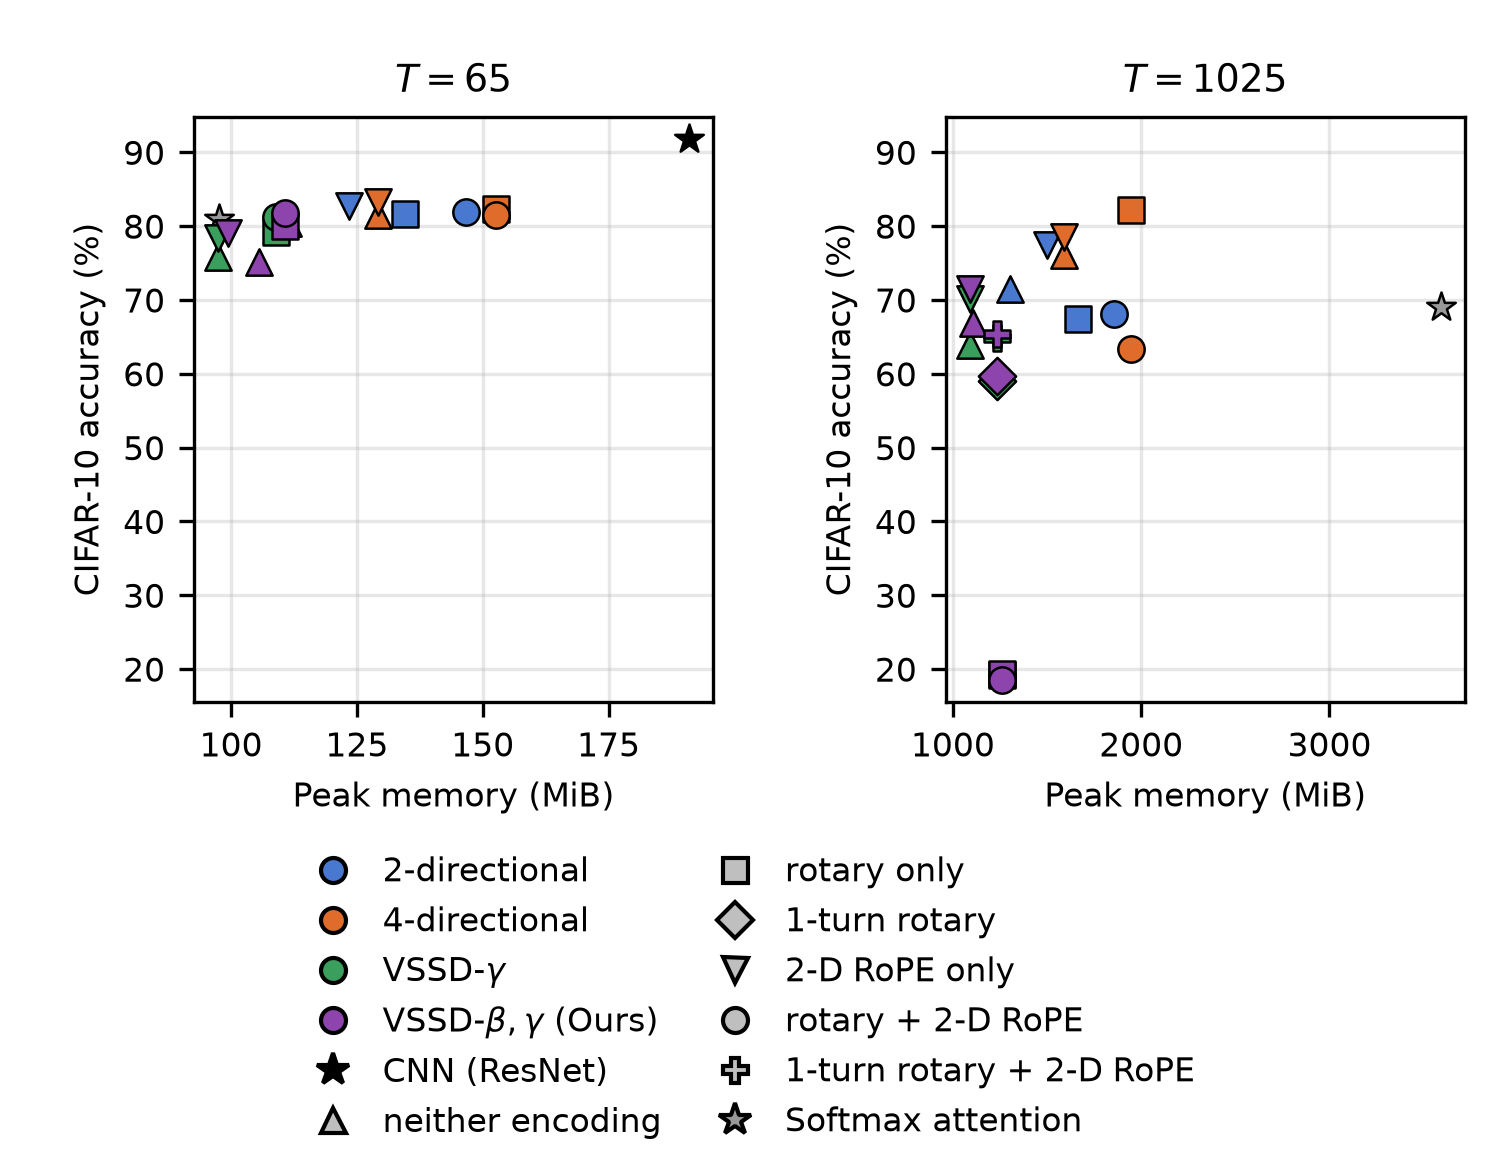
\includegraphics[width=\linewidth]{ablation_mem_acc.png}
\caption{Accuracy against peak memory, the trade-off the operators exist to
change; colour, marker, and baseline keys are given in the legend. Both panels share
one accuracy axis, so heights are directly comparable across sequence lengths; the
memory axes are independent, because peak memory differs by roughly $20\times$
between them and a shared one would collapse the $T{=}65$ panel to a line. At
$T{=}65$ memory is almost flat across operators and the plot is effectively an
accuracy ranking; at $T{=}1025$ the state-space operators separate from softmax
attention horizontally, which is the property the linear-time recurrence buys. The
shared axis is stretched by one point, VSSD-$\gamma$ with both encodings at $18.94$
(\S\ref{sec:ablation}), which compresses the rest. The CNN appears only in the
$T{=}65$ panel: it does not tokenise, so it has no token count for the right panel to
place it at, and its memory does not sit on the same scaling curve the panel is
about. Its numbers at both settings remain in Table~\ref{tab:ablation}.}
\label{fig:ablation-mem-acc}
\end{figure}

\paragraph{What the grid shows.}
The rotary-only column is the one that changes the reading, and the reason this grid is
a $2\times2$ per operator rather than three columns. As main effects and interaction at
$T{=}65$:

\begin{center}\small
\begin{tabular}{|l|cc|cc|}
\hline
Operator & rotary alone & 2-D RoPE alone & sum of the two & measured together \\ \hline
2-directional & $+1.15$ & $+2.34$ & $+3.49$ & $+1.45$ \\ \hline
4-directional & $+0.73$ & $+1.74$ & $+2.47$ & $-0.07$ \\ \hline
VSSD-$\gamma$ & $+3.39$ & $+2.64$ & $+6.03$ & $+5.42$ \\ \hline
\end{tabular}
\end{center}

Every entry in the first two columns is positive: \emph{both} encodings help
\emph{every} operator when it is the only one present. The rotary is therefore not
harmful to the scan operators --- which is exactly how its marginal deltas ($-0.89$
two-directional, $-1.81$ four-directional, $+2.78$ VSSD-$\gamma$) read when no
rotary-only cell exists to compare against, and is what an earlier draft of this
section concluded from precisely that missing column. What is negative is the
\emph{interaction}: measured-together minus sum-of-the-two is $-2.04$ two-directional
and $-2.54$ four-directional, against $-0.61$ for VSSD-$\gamma$, and that last figure
is inside the $0.67$ repeat spread, i.e.\ indistinguishable from the two encodings
simply adding. The encodings are individually useful everywhere, strongly redundant
with each other on the scan operators, and close to complementary on VSSD-$\gamma$.

That pattern is \emph{not} about position: the rotary's angle
$\theta_t=\bm{W}_\theta\bm{x}_t$ \eqref{eq:dtheta} is a function of a token's own
content only, never its index or grid location, so on its own it carries no
relative-position information at all. What it does carry is a query-specific rotation
of $\bm{C}_i$ before the readout, and how much that matters depends on how much
query-specific behaviour the operator already has elsewhere. The scan operators already
give every query its own full, per-pair interaction through the mask $L_{ij}$
\eqref{eq:L3}, so one more content-dependent knob is largely redundant complexity.
\S\ref{sec:ncssd-mamba3} shows VSSD-$\gamma$'s mask has instead collapsed to a single
shared summary $\bm{H}$ that every query reads identically, so rotating $\bm{C}_i$ by
its own content is close to the \emph{only} source of query-specific behaviour it has
--- which is why it helps so much. 2-D RoPE helps VSSD-$\gamma$ for a related reason and
also supplies what the rotary cannot: genuine relative-position information, which the
scan operators already had from their mask's decay in $|i-j|$ and VSSD-$\gamma$ had
none of at all. The two accounts together predict the interaction pattern above ---
redundant where the operator already has both properties, additive where it has
neither. VSSD-$\gamma$ moves $75.76 \to 81.18$ across its row. The implementation
defaults to each operator's best cell: the rotary on for VSSD-$\gamma$, off for the
scan operators, with 2-D RoPE on throughout.

Two things the grid does \emph{not} establish, both because of the $0.67$-point
repeat spread in the caption. Four-directional scanning is not shown to beat
two-directional: their best cells differ by $0.50$, inside the noise. And the
best cell overall, 4-directional with 2-D RoPE at $83.28$, leads softmax
attention by $2.36$ --- above the spread, but on a single seed at one recipe, so
it is a result to reproduce rather than to quote.

\paragraph{A trap worth recording.}
These numbers are the ones measured \emph{after} 2-D RoPE was corrected to pair
adjacent channels, matching the rotary's convention (\S\ref{sec:rope2d}). Before
that, the two encodings rotated in disjoint planes; each was self-consistent
alone, so single-encoding cells were unaffected, but with both enabled the
composition no longer reduced to a function of $i-j$. Measured as the departure of
the score matrix from Toeplitz on constant content, the violation was
$1.3\times10^{-2}$ against $2.2\times10^{-7}$ once matched --- five orders of
magnitude --- and it cost the 2-directional operator $12$ points: $70.2$ with both
encodings enabled, against $82.78$ with 2-D RoPE alone and $81.59$ with the rotary
alone.

All three single-encoding cells were re-measured under the corrected pairing, so
every cell of Table~\ref{tab:ablation} now comes from one operator build rather
than being carried over on the argument that the fix could not have touched them.
Two moved within the repeat spread ($82.71\to82.78$ two-directional,
$83.26\to83.28$ four-directional); VSSD-$\gamma$ moved $79.40\to78.40$, a full point,
slightly beyond it. That is broadly the ``unaffected'' the argument predicts, but
on single seeds it is corroboration rather than proof --- which is the reason for
re-running them instead of assuming.

The trap is worth recording because the broken configuration did not merely
underperform: for the
4-directional operator it \emph{over}-performed, reaching the best accuracy in the
whole grid, which is exactly the kind of result that survives review unexamined.

%% ================================================================
%% ================================================================
%% ================================================================
\subsection{Why the rotary destroys VSSD at long sequence length}
\label{sec:rotary-vssd}
%% ================================================================
The $T{=}1025$ half of the grid contains one result that no amount of tuning
explains away. With the rotary alone, both VSSD operators sit at $19.14\%$ and
$19.35\%$ against a $10\%$ chance floor, while the \emph{same} rotary makes
four-directional the best row in the table at $82.18\%$. Yet at $T{=}65$ that
encoding is worth $+3.39$ and $+4.87$ to those same VSSD operators --- more than it
gives any scan operator. The reversal is not a training accident: it follows from
what the collapse does to the keys.

\paragraph{What the angle actually is.}
\texttt{AttentionProjections} emits $N/2$ extra values per token, from the same
linear map that produces $\bm{B},\bm{C},\bm{V}$, so the per-token angle increment
$\varepsilon_j$ is \emph{learned} and data-dependent. Those rows are
zero-initialised, so the rotary is the identity at step $0$. The angle carried by
token $j$ is the running sum $\theta_j=\sum_{k\le j}\varepsilon_k$, and
\texttt{rotate\_pairs} turns adjacent channel pairs of $\bm{B}_j$ and $\bm{C}_j$ by
$(\cos\theta_j,\sin\theta_j)$. This is unlike a classical RoPE, whose angle is a
\emph{fixed} function of position on a geometric frequency schedule; here it is
learned and cumulative, and that is what makes its spread depend on $T$.

\paragraph{Why it works in the scans.}
Rotating $\bm{B}$ and $\bm{C}$ by their own angles makes a score depend only on the
difference,
\begin{equation}
  \bigl(\mathcal{R}(\theta_i)\bm{C}_i\bigr)^{\!\top}\bigl(\mathcal{R}(\theta_j)\bm{B}_j\bigr)
  = \bm{C}_i^{\top}\,\mathcal{R}(\theta_i-\theta_j)\,\bm{B}_j ,
  \label{eq:rotary-relative}
\end{equation}
because a rotation is orthogonal. The absolute angle cancels; only the relative one
survives, which is the whole point of a rotary embedding. Note what
\eqref{eq:rotary-relative} requires: the inner product must be formed \emph{before}
any summation over $j$. The SSD form \eqref{eq:ssd} does exactly that, one score per
pair, and nothing about it degrades as $T$ grows --- which is why four-directional
with the rotary is the best $T{=}1025$ row rather than a casualty.

\paragraph{Why VSSD is different, and why the rotary still helps it most.}
The collapse forms no pairwise score at all. Equation~\eqref{eq:vssd} sums the keys
into a single state before any query is involved,
\begin{equation}
  \bm{H}=\sum_j m_j\,\bigl(\mathcal{R}(\theta_j)\bm{B}_j\bigr)\otimes\bm{V}_j ,
  \qquad
  \bm{Y}_i=\bigl(\mathcal{R}(\theta_i)\bm{C}_i\bigr)^{\!\top}\bm{H},
  \label{eq:vssd-rotary}
\end{equation}
which is precisely what buys $O(T)$ instead of $O(T^2)$. No $\theta_i-\theta_j$ ever
appears, so \eqref{eq:rotary-relative} is unavailable by construction. The rotary is
nevertheless the most valuable encoding VSSD has, by a different route: $\bm{C}_i$ is
rotated too, so query $i$ reads the one pooled state along a direction set by its own
position. Without it the read-out cannot depend on $i$ at all, because $m_j$ carries
no query index --- the asymmetry of \S\ref{sec:ncssd-mamba3} --- and that is why
$+3.39$ and $+4.87$ exceed anything the scans gain.

\paragraph{What breaks at $T{=}1025$.}
The failure is in $\bm{H}$, not in the read-out. Each token contributes
$m_j\mathcal{R}(\theta_j)\bm{B}_j$ and those are \emph{summed}. Within each of the
$N/2$ rotation planes the contributions are vectors turned by $\theta_j$; if the
$\theta_j$ span many full turns they point in effectively unrelated directions, and
the sum grows like $\sqrt{T}$ rather than $T$ --- a shortfall of about $32\times$ at
$T{=}1025$. Training aligns the $\bm{B}_j$ so their sum carries signal; a wide spread
scrambles that alignment, and the state every query reads becomes noise. Because
$\theta$ is a plain running sum, the spread is $T\varepsilon$: roughly ten full turns
at $T{=}65$, roughly $160$ at $T{=}1025$.

\paragraph{Why training does not simply learn a smaller angle.}
This is the natural objection --- the increments are learned, so the optimiser should
pick a value that works. Two things prevent it, and the second is why it cannot
recover.

The running sum welds together two quantities that must be set independently. The
resolution between \emph{neighbouring} tokens is $\varepsilon$ itself, while the
spread across the \emph{whole} sequence is $T\varepsilon$. They share one parameter
and their ratio is fixed at $T$, so an $\varepsilon$ large enough to distinguish
adjacent tokens forces a spread $T$ times larger. At $T{=}65$ both can hold at once;
at $T{=}1025$ no value satisfies both.

The gradient reaching those rows is amplified by the same running sum. Since
$\partial\theta_j/\partial\varepsilon_k=1$ for every $j\ge k$, each increment collects
the gradient of every later position --- up to $1025$ terms against $65$. The angles
begin at zero, which is the identity and hence the \emph{good} configuration, and this
amplified gradient carries them out of it inside the first epoch. Once $\bm{H}$ has
decohered the loss is flat at chance, so no gradient points back. The logs show
exactly this: training loss $2.21$ at epoch~1 against $\ln 10=2.303$, still $2.26$ at
epoch~6, while the same operator with no encoding falls $1.97\to1.57$ over five.

\paragraph{Confirmation.}
If the spread is the cause, bounding it must restore training with nothing else
changed. Scaling the per-token increment by $65/1025$ gives $T{=}1025$ exactly the
spread $T{=}65$ had (\texttt{--rope-angle-scale}, VSSD-$\gamma$, six epochs):
\begin{center}\small
\begin{tabular}{|l|cc|cc|}
\hline
$T{=}1025$, VSSD-$\gamma$ & ep.\ 1 & ep.\ 3 & ep.\ 6 & test \\ \hline
rotary, unscaled ($\sim$$160$ turns) & $2.26$ / $15.2\%$ & $2.19$ / $16.5\%$ & $2.26$ / $13.6\%$ & $14.6\%$ \\ \hline
rotary, scaled ($\sim$$10$ turns) & $1.90$ / $30.3\%$ & $1.66$ / $39.6\%$ & $1.65$ / $39.6\%$ & $42.7\%$ \\ \hline
no encoding (reference) & $1.97$ / $27.1\%$ & $1.75$ / $35.7\%$ & --- & --- \\ \hline
\end{tabular}
\end{center}
It does. The mechanism is therefore confirmed: bounding the spread turns a total
collapse into ordinary training, with nothing else changed.

What it does \emph{not} do is make the rotary worth using at this length, and the
full runs say so plainly. At $30$ epochs with the spread pinned to one turn
(Table~\ref{tab:ablation}, the \texttt{1-turn} rows):
\begin{center}\small
\begin{tabular}{|l|cc|cc|}
\hline
$T{=}1025$ & no encoding & 1-turn rotary & 2-D RoPE & 1-turn rotary $+$ 2-D RoPE \\ \hline
VSSD-$\gamma$ & $63.88$ & $58.98$ & $\mathbf{70.10}$ & $64.83$ \\ \hline
VSSD-$\beta,\gamma$ & $66.90$ & $59.69$ & $\mathbf{71.44}$ & $65.44$ \\ \hline
\end{tabular}
\end{center}
The repair is worth $+40$ points against the collapsed cells ($19.14$ and $19.35$),
and $+46$ where both encodings are on ($18.94$ and $18.47$). But the bounded rotary
alone still trails \emph{no encoding at all}, and adding it to 2-D RoPE still costs
five to six points against 2-D RoPE alone. It stops destroying the model without
becoming useful.

The six-epoch probe above suggested otherwise --- there the bounded rotary led the
no-encoding reference --- and that advantage does not survive to convergence. We
report the longer runs, since they are the ones the rest of the grid is measured at.
The practical conclusion is unchanged and now measured rather than inferred: at long
sequence length, 2-D RoPE alone.

\paragraph{The remedy, and what in it is ours.}
If the spread is the whole problem, the fix is to stop letting it depend on $T$: the fixed
$n$-turn angle $\theta_j=2\pi n j/T$ of \eqref{eq:rope-turns}, derived in
\S\ref{sec:rope-turns}, which removes the coupling outright rather than balancing it.
Sweeping $n$ on VSSD-$\gamma$ at $T{=}1025$ (six epochs, test accuracy) is monotone in
favour of less spread:
\begin{center}\small
\begin{tabular}{|l|c|c|c|c|}
\hline
total spread & $\sim$$1$ turn & $\sim$$10$ turns & $\sim$$163$ turns (learned) & no encoding \\ \hline
test acc. & $\mathbf{51.9\%}$ & $42.7\%$ & $14.6\%$ & $\sim$$36\%$ \\ \hline
\end{tabular}
\end{center}

\noindent\textbf{Equation~\eqref{eq:rope-turns} is not new and we do not claim it.} Dividing
a rotary's angle by the sequence length is Positional Interpolation~\cite{posinterp}, whose
$f'(x,i)=f(x,\,iL/L')$ is the same operation, and YaRN~\cite{yarn} and the NTK-aware
variants refine it further. Even the trade-off is known there: interpolating too far
``prevent[s] models from distinguishing nearby positions'', which is exactly why shrinking
the spread must eventually degenerate toward no encoding at all.

What we believe is not documented is the \emph{reason it is needed here}, and the
difference matters. Positional Interpolation addresses \emph{length extrapolation}: a model
trained at $L$ and evaluated at $L'>L$ sees position indices it never met, and rescaling
brings them back into the trained range. Our failure is not extrapolation. The $T{=}1025$
model is \emph{trained} at $T{=}1025$ and never sees a shorter sequence; nothing is being
extrapolated, and no rescaling is restoring a familiar range. What is being repaired is the
coherence of a \emph{pooled} state --- a quantity that has no counterpart in pairwise
attention, where every rotation meets a query and cancels. So the same arithmetic is
serving a different purpose, and the condition it enforces is different too: not ``keep
positions inside the trained range'' but ``keep the total spread $O(1)$ turns, at every
length, including the one you trained on''.

We state this as a mechanism we have not seen reported rather than as a novelty claim; a
literature search is weak evidence of absence, and the arithmetic itself is certainly
prior art.

\paragraph{Why 2-D RoPE is safe for every operator at both lengths.}
Its angle is $\theta_{r,c}[n]=\theta^{\mathrm{row}}[n]\,r+\theta^{\mathrm{col}}[n]\,c$,
a function of the patch's position on the image grid, so it is bounded by the image
rather than growing with the sequence. Bounded angles survive pooling; accumulated
ones do not. That one distinction accounts for 2-D RoPE being the only encoding that
helps every operator at both sequence lengths, and it is why we deploy it alone at
long $T$.

\paragraph{Two dead ends, recorded so they are not retried.}
Wrapping $\theta$ into $[-\pi,\pi)$ changes nothing, since $\cos$ and $\sin$ are
$2\pi$-periodic: the rotation already depends only on $\theta$ modulo $2\pi$, and the
\emph{spread} is what matters. And the missing $\Delta$ is not the cause on its own.
The SSD path accumulates $\mathrm{cumsum}(\text{angles}\cdot\Delta)$ while the
collapse accumulates $\mathrm{cumsum}(\text{angles})$, $\Delta$ having not survived
the reduction (\S\ref{sec:ncssd-mamba3}); but the measured $\Delta$ is about $0.74$,
giving $758$ radians against $1025$ at $T{=}1025$ --- a factor of $1.35$, which cannot
separate the best row in the table from total collapse.

\section{Application 3: Mamba-3 for Pose Estimation}
\label{sec:eth3d}
%% ================================================================

\emph{Two different ETH3D experiments exist in this project and are easy to
confuse.} This section is the \textbf{camera-pose} one, scored by
AUC@30\textdegree, and it failed. \S\ref{sec:eth3d-depth} is the
\textbf{metric-depth} one, scored by abs.\ rel.\ / RMSE / $\log_{10}$ /
$\delta{<}1.25$, and that is the experiment the paper's depth table reports.
They use different scene splits, different losses and different metrics, so a
result from one carries no information about the other.

We swapped the attention modules in DA-3-SMALL ($16$ layers total: 12
backbone + 4 camera-encoder) and trained with GT-supervised
multi-scene loss on a random scene split (seed=42) of all 11 extracted
ETH3D scenes: 8 train / 3 held-out test. Recipe and split mirror the
existing \S15.59.8 protocol so SSD and VSSD are directly comparable.

\subsection{Setup (\texorpdfstring{\S}{Sec.}15.59.8 protocol, identical for SSD and VSSD)}

\begin{center}
\begin{tabular}{ll}
\toprule
Dataset / scenes      & ETH3D, 11 scenes, 8 train / 3 test (seed 42) \\
Test scenes           & courtyard, delivery\_area, terrains \\
Init                  & random (\texttt{install\_mamba3} default init) \\
Steps                 & 3000 (warmup 100, decay 500) \\
LRs                   & attn=1e-5, head=5e-5, other=1e-5 \\
Loss                  & original DA-3 paper $c\cdot|err| - \lambda\log(c)$ \\
Image size            & 504 \\
Views per step        & 4 \\
Checkpoint every      & 500 steps \\
Metric                & AUC@30$^\circ$ (pose), mean across 3 test scenes \\
\bottomrule
\end{tabular}
\end{center}

\subsection{Results -- both Mamba variants fail to beat zero-shot}

\begin{center}\small
\begin{tabular}{lrrl}
\toprule
Variant & Best mean AUC@30$^\circ$ & Best at ckpt & Trajectory \\
\midrule
DA-3-SMALL zero-shot$^{\dagger}$ & $\sim 0.66$ (terrains)$^*$ & -- & -- \\
DA-3 + Mamba-3 SSD & $\approx 0.006$ & 2500 & flat near 0 \\
DA-3 + Mamba-3 VSSD & \textbf{0.0645} & 500 & peak then decline \\
\bottomrule
\end{tabular}
\end{center}

\noindent{\footnotesize $^{\dagger}$Un-patched, no training. Both Mamba rows are
trained from random init at lr $10^{-5}$, per the recipe above.}

\noindent$^*$ Published reference in PLAN.md \S15.59 -- DA-3-SMALL
zero-shot on \texttt{terrains}. A 3-scene reproduction was attempted
but the un-patched DA-3 zero-shot eval on \texttt{terrains} hangs in
the same TSDF retry loop as some trained variants (degenerate-depth
preflight); the published per-scene number is used here.

\paragraph{Reading the table.}
\begin{itemize}
  \item \textbf{Both trained variants fail catastrophically.} Even
        VSSD's peak ($0.0645$) is $\sim 10\times$ below DA-3 zero-shot
        ($\sim 0.66$). Training from random init at this recipe
        \emph{actively hurts} the model relative to using the
        pretrained DA-3-SMALL weights as-is.
  \item \textbf{Relative to SSD, VSSD is $\sim 10\times$ better in
        absolute terms} (peak $0.0645$ vs $\sim 0.006$). VSSD peaks
        early (ckpt 500) and degrades monotonically afterwards;
        SSD is flat near zero from the start.
  \item \textbf{The recipe-robustness observed on CIFAR-10 partly
        transfers.} On CIFAR's cosine recipe VSSD beat SSD by
        $+32.7$~pp without collapsing; on ETH3D's lr1e5 recipe VSSD
        again \emph{visibly trains} (a peak exists) while SSD
        produces flat-zero metrics. But both still over-fit hard:
        VSSD's training loss drove to $-14$ (the model collapses
        toward "no confidence" predictions to satisfy the
        $-\log(c)$ aleatoric term) while test loss climbed from
        $18$ to $40$ over the same window.
\end{itemize}

\paragraph{Diagnosis.}
The DA-3 task is fundamentally different from CIFAR-10 in two ways
that both work against from-scratch Mamba initialisation: (i) the
DA-3 head consumes pretrained backbone features that were optimised
for softmax attention; random Mamba-3 attentions destroy those
features within the first $\sim 100$ steps before any compensating
signal arrives; (ii) the DA-3 paper loss is not regularised against
the depth-saturation degeneracy that the from-scratch Mamba init
falls into. PLAN.md \S15.59.8 identifies the same failure mode
under SSD and proposes feature distillation from a frozen teacher
(\S15.59.5 plan) or recipe changes as the next steps. VSSD's
recipe-robustness gain alone is not enough to close the gap; the
init problem is the bottleneck.

%% ================================================================
%% ================================================================
%% ================================================================
\section{Application 4: Mamba-3 for Metric Depth Estimation}
\label{sec:eth3d-depth}
%% ================================================================

This is the experiment behind the depth table in the paper. It is separate from
the pose experiment of \S\ref{sec:eth3d} in every respect: different split,
different loss, different metrics.

\subsection{Scene split -- what is trained on and what is not}
\label{sec:eth3d-depth-split}

The split is by \textbf{scene}, fixed, and not random. Of the 11 extracted
ETH3D scenes that carry ground-truth depth:

\begin{center}
\begin{tabular}{ll}
\toprule
\textbf{Train} (10 scenes, 374 images) &
  \texttt{courtyard}, \texttt{delivery\_area}, \texttt{electro},
  \texttt{facade}, \texttt{kicker}, \\
 & \texttt{office}, \texttt{pipes}, \texttt{playground},
  \texttt{relief}, \texttt{relief\_2} \\
\midrule
\textbf{Held out} (eval only) & \texttt{terrains} (42 views) \\
\bottomrule
\end{tabular}
\end{center}

\noindent\textbf{\texttt{terrains} is never trained on, in either phase.} Both
the distillation phase and the depth fine-tune draw only from the 10 training
scenes; \texttt{terrains} is touched exclusively by the evaluator. Any future
change to this harness must preserve that, and a run that cannot demonstrate it
should not be reported.


\begin{figure}[!tb]
\centering
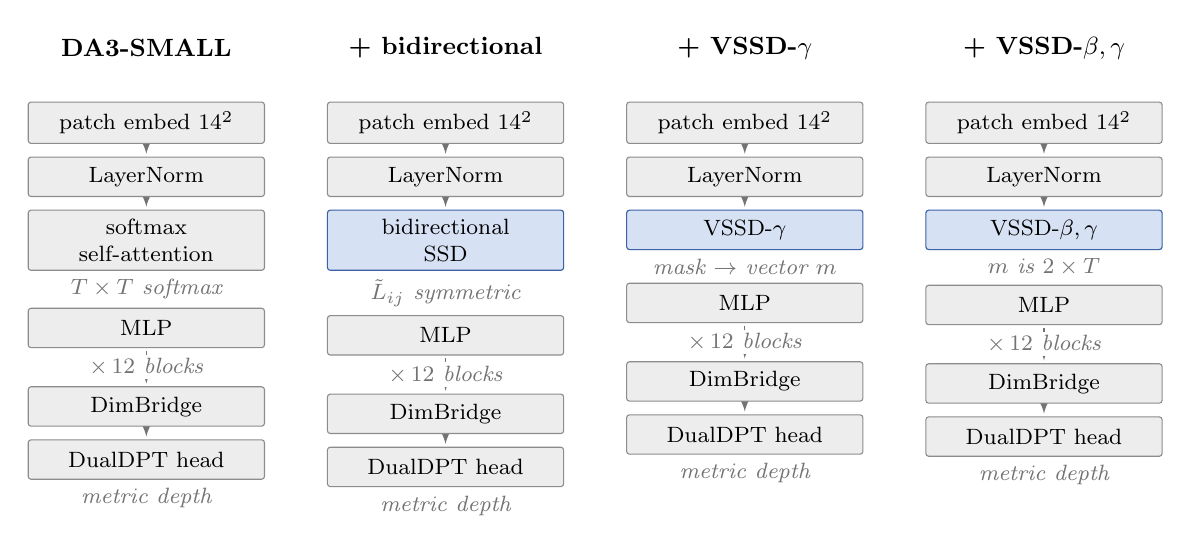
\begin{tikzpicture}[
  font=\footnotesize,
  bx/.style   = {draw=black!45, fill=black!7,  rounded corners=1pt,
                 minimum width=30mm, minimum height=5.0mm, align=center},
  tr/.style   = {draw=cTrain!80!black, fill=cTrain!22, rounded corners=1pt,
                 minimum width=30mm, minimum height=5.0mm, align=center},
  % \footnotesize, not \scriptsize: the paper's font floor forbids anything smaller,
  % and this figure should stay liftable into it. Hierarchy comes from colour and
  % italics instead of size. White fill so the "x 12 blocks" note masks the arrow it
  % sits on rather than overprinting it.
  note/.style = {font=\footnotesize\itshape, text=black!55, align=center,
                 fill=white, inner sep=1.2pt},
  hd/.style   = {font=\small\bfseries, align=center},
  ar/.style   = {-latex, draw=black!55, shorten >=1pt, shorten <=1pt},
]
\def\colsep{38mm}
\foreach \i/\name/\mix/\mixsty/\mask in {
  0/{DA3-SMALL}/{softmax\\self-attention}/bx/{$T\times T$ softmax},
  1/{+ bidirectional}/{bidirectional\\SSD}/tr/{$\tilde L_{ij}$ symmetric},
  2/{+ VSSD-$\gamma$}/{VSSD-$\gamma$}/tr/{mask $\to$ vector $m$},
  3/{+ VSSD-$\beta,\gamma$}/{VSSD-$\beta,\gamma$}/tr/{$m$ is $2\times T$}}
{
  \begin{scope}[xshift=\i*\colsep]
    \node[hd]                          (h\i) at (0,0.95) {\name};
    \node[bx]                          (pe\i) at (0,0)      {patch embed $14^2$};
    \node[bx, below=1.6mm of pe\i]     (ln\i) {LayerNorm};
    \node[\mixsty, below=1.6mm of ln\i](mx\i) {\mix};
    \node[note, below=0.6mm of mx\i]   (nt\i) {\mask};
    \node[bx, below=0.6mm of nt\i]     (mlp\i){MLP};
    \node[note, below=0.8mm of mlp\i]  (xn\i) {$\times\,12$ blocks};
    \node[bx, below=0.8mm of xn\i]     (br\i) {DimBridge};
    \node[bx, below=1.6mm of br\i]     (dp\i) {DualDPT head};
    \node[note, below=0.6mm of dp\i]         {metric depth};
    % Background layer: the "x 12 blocks" note is white-filled to mask the arrow it
    % sits on, which only works if the arrow is drawn underneath it.
    \begin{pgfonlayer}{background}
      \foreach \a/\b in {pe\i/ln\i, ln\i/mx\i, mlp\i/br\i, br\i/dp\i}
        \draw[ar] (\a) -- (\b);
    \end{pgfonlayer}
  \end{scope}
}
\end{tikzpicture}
\caption{The four backbones compared on ETH3D metric depth
(\S\ref{sec:eth3d-depth}). Only the self-attention mixer inside DA3-SMALL is
swapped; patch embedding, MLPs and DimBridge keep DA3-SMALL's pretrained
weights in every column. \textcolor{cTrain!80!black}{\textbf{Blue}} marks what
\emph{Phase B} trains: the mixer alone, with everything grey frozen at DA3-SMALL's
pretrained values for those $11\,000$ steps. Phase C then unfreezes the entire
network (\S\ref{sec:eth3d-depth-protocol}), so this colouring describes the
distillation phase, not the final state. DA3-SMALL is the zero-shot reference,
so nothing in its column is trained at all. The
three swapped columns differ \emph{only} in the mask their mixer applies, noted
under each: a symmetric $|i-j|$ decay for the bidirectional scan, a single
per-token vector for VSSD-$\gamma$, and two independently-read pools for
VSSD-$\beta,\gamma$.}
\label{fig:depth-variants}
\end{figure}

\subsection{Two-phase protocol}
\label{sec:eth3d-depth-protocol}

\paragraph{Phase B -- feature distillation (20\,000 steps).}
The student is DA3-SMALL with its self-attention replaced by Vision Mamba-3;
everything else is DA3-SMALL's pretrained weights. The teacher is the
\emph{unmodified} DA3-SMALL, frozen. The loss matches student to teacher
features (L2 $+$ cosine) at backbone layers $(5,7,9,11)$ of 12,
$d_{\text{embed}}=384$. Images at $504^2$, batch 1, chunked SSD
(\texttt{chunk\_size}=128), lr $3\times10^{-4}$. Augmentation: random crop
0.6--1.0, horizontal flip $p=0.5$, colour jitter $\pm0.4/0.1$.

\paragraph{Phase C -- GT-supervised depth fine-tune (1\,000 steps).}
Initialised from the Phase-B checkpoint. Loss is SILog (scale-invariant
log-RMSE) $+$ edge-aware smoothness against ground-truth depth on the 10
training scenes. Cosine schedule ending near zero LR at step 1000; bf16
autocast. Learning rates by group:
\[
  \text{lr}_{\text{attn}} = 10^{-5}, \qquad
  \text{lr}_{\text{bridge}} = 3\times10^{-5}, \qquad
  \text{lr}_{\text{dpt}} = 10^{-5}.
\]

\noindent\textbf{The DualDPT depth head is unfrozen in Phase C.} This is
deliberate --- unfreezing it is the single change that produced the result --- but
it must be stated whenever the numbers are quoted, because it invalidates the
tempting claim that the head is frozen at DA3-SMALL's own calibration and that
matching DA3-SMALL is therefore the best achievable outcome by construction.
That ceiling argument describes an \emph{earlier} recipe, in which the head was
frozen; it does not describe this one.

\paragraph{Recipe at a glance.} The two phases differ in \emph{what is allowed
to move}, and that difference is the single thing most often misread, so it is
tabulated rather than left in prose. Counts are for VSSD-$\beta,\gamma$; the
one-pool operators have a $11.61$\,M mixer and $36.45$\,M total.

\begin{center}
\begin{tabular}{lll}
\toprule
 & \textbf{Phase B} (distillation) & \textbf{Phase C} (depth fine-tune) \\
\midrule
Steps        & $11\,000$ (CM12/CM24 used $20\,000$) & $1\,000$ \\
Trainable    & the swapped mixer, and nothing else  & \emph{the whole network} \\
             & $15.03$\,M of $39.86$\,M             & $39.86$\,M of $39.86$\,M \\
Frozen       & patch embed, MLPs, DimBridge,        & nothing \\
             & DualDPT, \texttt{cam\_enc}           & \\
Breakdown    & attn $15.03$                          & attn $15.03$, dpt $0.44$, \\
             &                                       & \texttt{cam\_dec} $1.19$, other $23.21$ \\
Supervision  & a frozen teacher's features           & ETH3D ground-truth depth \\
Teacher      & DA3-SMALL (dim-matched, L2$+$cos) or  & none \\
             & DA3-LARGE (token-Gram, dim-free)      & \\
Data         & \multicolumn{2}{l}{$39$ train scenes: ETH3D $10$, HiRoom $25$, 7-Scenes $4$
                 --- \texttt{terrains} excluded from both} \\
\bottomrule
\end{tabular}
\end{center}

\noindent Two consequences follow, and both contradict readings that are easy to
reach from the phase names alone. Phase C leaves \emph{nothing} frozen --- the
$23.21$\,M ``other'' is the patch embedding, the MLPs and DimBridge, so the
network is free to co-adapt to whatever features Phase B produced, not merely to
re-fit a head on top of them. And the two budgets are asymmetric by $11\times$:
whatever Phase B settles into under the constraint that only the mixer may move,
Phase C has a tenth of the steps to move away from. A recipe whose Phase-B target
is a poor one is therefore not rescued by Phase C being unconstrained, which is a
budget property and not a structural limit --- a longer Phase C has never been
tried.

\subsection{Evaluation}
\label{sec:eth3d-depth-eval}

All four metrics are computed on the 42 held-out \texttt{terrains} views, after
per-image median scale alignment of prediction to ground truth: absolute
relative depth error, RMSE, $\log_{10}$, and $\delta{<}1.25$ (all except RMSE
median-aligned; the acceptance gate for RMSE is defined on the raw value).

\paragraph{The baseline is zero-shot.} DA3-SMALL is evaluated off the shelf,
with no ETH3D training of any kind. Our student has 20\,000 distillation steps
plus 1\,000 GT-supervised steps on ETH3D's other 10 scenes. This is a
fine-tuned-versus-zero-shot comparison across disjoint scenes of one dataset ---
a legitimate transfer setup, and \emph{not} train-on-test --- but it is not a
like-for-like backbone comparison, and reporting it as one would overstate the
result. It is the reason our student can lead on $\delta{<}1.25$ while trailing
on the other three metrics.

\subsection{Reference numbers (legacy run)}
\label{sec:eth3d-depth-legacy}

The numbers currently in the paper come from the run recorded as CM22@1000 in
the retired \texttt{largescale3Dreconstruction\_\allowbreak{}using\_\allowbreak{}SSM} repository
(pipeline \texttt{distill\_\allowbreak{}cm12/\allowbreak{}ckpt\_\allowbreak{}20000.pt} $\rightarrow$
\texttt{depth\_\allowbreak{}ft\_\allowbreak{}cm22/\allowbreak{}ckpt\_\allowbreak{}1000.pt}, 2026-04-23):

\begin{center}
\begin{tabular}{lcccc}
\toprule
 & abs.\ rel.\,$\downarrow$ & RMSE\,$\downarrow$ & $\log_{10}$\,$\downarrow$ & $\delta{<}1.25$\,$\uparrow$ \\
\midrule
DA3-SMALL (zero-shot)     & \textbf{0.0417} & \textbf{0.0796} & \textbf{0.0175} & 0.9743 \\
Vision Mamba-3 (CM22@1000) & 0.0531 & 0.1012 & 0.0229 & \textbf{0.9972} \\
\bottomrule
\end{tabular}
\end{center}

\noindent These predate the operator update: they were produced \emph{without}
2-D RoPE and against an older \texttt{mamba-ssm} kernel. They are recorded here
as the reference to reproduce, not as a current result.

\subsection{What this repository provides}
\label{sec:eth3d-depth-harness}

The harness is being ported into this repository from the retired repo's
\texttt{mamba3\_attn} package, so that the experiment is reproducible from a
single checkout rather than from a repository that no longer exists. The pieces
and their roles:

\begin{itemize}
  \item \textbf{DA3 patching} (\texttt{da3\_adapter.py}, \texttt{patch.py}) ---
        swaps DA3-SMALL's self-attention for the Vision Mamba-3 operator
        (implementation notes: \S\ref{sec:impl}), leaving every other weight at its pretrained value.
  \item \textbf{ETH3D loaders} (\texttt{data/eth3d.py},
        \texttt{data/eth3d\_\allowbreak{}multi.py}) --- scene discovery, GT-depth pairing,
        and the fixed split of \S\ref{sec:eth3d-depth-split}.
  \item \textbf{Training phases} (\texttt{train/train\_\allowbreak{}super.py}) --- Phase B is
        \texttt{-{}-super 1} (DA3-SMALL teacher), Phase C is
        \texttt{-{}-super 3 -{}-sub 3} (GT supervision, full unfreeze), matching
        the recipe of \S\ref{sec:eth3d-depth-protocol}.
  \item \textbf{Depth metrics} (\texttt{eval/metrics.py}) ---
        \texttt{abs\_\allowbreak{}relative\_\allowbreak{}depth\_\allowbreak{}error}, \texttt{rmse},
        \texttt{log10\_metric}, \texttt{delta\_threshold}, and
        \texttt{align\_\allowbreak{}scale\_\allowbreak{}median} for the alignment above.
\end{itemize}

The operator itself is \emph{not} ported: the patched DA3 uses this
repository's current \texttt{visionmamba3} modules, so the re-run measures the
updated operator (2-D RoPE, fused Triton kernel, pinned upstream submodule)
rather than the 2026-04 snapshot that produced the legacy numbers above.

%% ================================================================
\section{Conclusion}
%% ================================================================

%% ================================================================
\subsection{What the derivation gives}
%% ================================================================

Using only \eqref{eq:ssd-derived}, we have obtained:

\begin{itemize}
  \item \textbf{Self-attention:} \eqref{eq:self-out} and, with the
        content-based rotary, \eqref{eq:self-rope}. Multi-head via
        \eqref{eq:mimo-self}.
  \item \textbf{Cross-attention:} Variant~A \eqref{eq:crossA-out}
        (cheap, compressed KV) and Variant~B \eqref{eq:crossB-out}
        (exact).
  \item \textbf{Image encoder:} patchify + bidirectional /
        multi-direction SSD self-attention
        (\eqref{eq:bidi2},\eqref{eq:bidi4}) with 2-D RoPE
        \eqref{eq:rope2d}.
  \item \textbf{Multi-view encoder:} alternating within-view
        \eqref{eq:cvout}-style blocks and cross-view
        \eqref{eq:Lxview} blocks; or the compressed-state cross
        block \eqref{eq:crossA-out} when one side dominates.
  \item \textbf{VSSD-$\gamma$:} reinterpret $A_t$ as a
        current-token weight to obtain \eqref{eq:nc-Y},
        $\bm{Y} = \bm{C}\bigl((\bm{B}\odot\bm{m})^\top\bm{X}\bigr)$,
        which collapses the $T\times T$ mask $\bm{L}$ to a
        $T$-vector $\bm{m}$, removes causality without multi-scan,
        and yields the VSSD image block (Section~\ref{sec:ncssd}).
\end{itemize}

Every output formula above is a direct application of the single
identity
\begin{equation*}
  \bm{Y} = (\bm{L}\odot\bm{C}\bm{B}^\top)\bm{X},
\end{equation*}
which we derived from the Mamba-3 recurrence in
Section~\ref{sec:ssd}. The choices made by a specific architecture
amount to (i) which tokens supply $\bm{B},\bm{C},\bm{X}$ (self vs
cross vs multi-view), and (ii) which structured mask $\bm{L}$ is used
(causal vs bidirectional vs block-diagonal vs view-masked). Mamba-3's
exponential-trapezoidal rule \eqref{eq:L3} and complex-SSM rotary
\eqref{eq:complex-rec} then give the mask and the query/key its final,
expressive form.

%% ================================================================
\subsection{What the experiments show}
%% ================================================================

\begin{itemize}
  \item \textbf{Implementation cost is small.} Given an existing
        Mamba-3 SSD attention library, adding the VSSD variant was
        $\sim 150$ lines of new operator code, a thin adapter wrapper,
        a dispatch flag, plus eval-script auto-detect for ckpt
        loading. The structural identity \eqref{eq:duality} carries
        the implementation through with no architectural changes.
  \item \textbf{On CIFAR-10, VSSD's efficiency win is unconditional}
        ($\sim 1.5\times$ faster than SSD, $17\%$ less peak memory,
        matches softmax memory to within $0.3$ MiB) and its accuracy
        is much more \emph{recipe-robust} than SSD's. SSD only
        beats VSSD on accuracy when the recipe is specifically tuned
        for SSD; on off-the-shelf settings, VSSD is the more
        forgiving operator. Neither beats CNN at this data scale +
        recipe, as expected.
  \item \textbf{On ETH3D, the operator change alone is not enough.}
        Both Mamba-3 variants fail to beat un-patched DA-3 zero-shot
        from random init under the \S15.59.8 recipe. VSSD is
        substantially better than SSD in relative terms ($10\times$
        higher peak) but still $10\times$ worse than zero-shot in
        absolute terms. The likely root cause is the random Mamba
        initialisation destroying pretrained DA-3 features faster
        than the training loss can repair them.
  \item \textbf{Next steps for the ETH3D direction.} Feature
        distillation against a frozen DA-3-LARGE teacher
        (PLAN \S15.59.5) is the path that gives Mamba attention a
        pretrained-equivalent init. The VSSD operator slots into
        that pipeline unchanged via
        \texttt{install\_\allowbreak{}mamba3(..., variant="vssd")}.
\end{itemize}

\bibliographystyle{plain}
\bibliography{references}

\end{document}
